\addchapheadtotoc
\chapter{Solver Performance}\label{chapter:Example}
% The complexity of the radiation solver resulting from both its theoretical foundation as well as its computational implementation calls for 
%Correctly implementing a radiation solver can be difficult due to both the complex formulation behind radiation and the high dimensionality associated with the problem (6 dimensions: 3 in space, 2 in direction, and 1 in wavelength). Mistakes in the implementation may result in significant performance loss or inaccurate results. As such, 
An extensive series of validation and performance studies are conducted in this chapter to demonstrate the effectiveness and efficiency of the present radiation solver. 
Four test geometries are presented for verification and profiling using the methods discussed in section~\ref{section:SummaryOfSolvers}. 
% The new MCRT models using the bounding volume hierarchy approach are referred to as MCRT-ArborX, and the model without the BVH is referred to as MCRT-Standard. A well-established Fortran implementation is also used for verification and is referred to as MCRT-Fort.
The configurations include the canonical one-dimensional plane-parallel medium, a snapshot of large-eddy simulations of a three-dimensional backward-facing step combustor, a snapshot of a direct numerical simulation of a small turbulent pool fire, and a transient small turbulent pool fire. 
The plane-parallel simulation results are compared against the exact solutions presented in section~\ref{section:SolutionsToRTE} as a verification. The three solver implementations presented in section~\ref{section:SummaryOfSolvers} are used: Standard-Forward, ArborX-Reverse, and Hybrid-Reverse. These three are considered the most-likely candidates for maximized MCRT performance. The best performing method is then used for the remaining studies.



\section{One dimensional plane-parallel medium}
The plane-parallel medium is a simple, one dimensional case commonly used to verify radiation solvers. As shown in Fig.~\ref{fig:PlaneParallel2}, the geometry consists of two parallel plates surrounding a homogeneous radiatively-emitting and absorbing medium. The blue boundaries are cold, black walls, i.e., they emit negligible radiation but absorb all incident radiation, and the red boundaries are symmetry boundary conditions. The boxes in Fig.~\ref{fig:PlaneParallel2} are coarsened representations of the actual cell discretization used in the study. Under present conditions, discretization of $1000$ cells in the direction normal to the blue boundary and one cell in the off-normal directions are used. A uniform absorption coefficient and temperature is assigned to the cells, and the medium is frozen in time and simulated for one snapshot. Verification is conducted against the exact solution presented in section~\ref{section:SolutionsToRTE}. 
The configuration is first tested under a variety of absorption coefficients and temperatures.
The MCRT solution procedure is repeated $50$ times for each condition, and $1000$ means and standard deviations are calculated for each of the $1000$ computational cells in the 1-D domain.
Results from all three primary methods listed in section~\ref{section:SummaryOfSolvers} are tested: Standard-Forward, ArborX-Reverse, and Hybrid-Reverse. First for a single MPI rank and then within multiple MPI ranks. Finally, the effect of varying ray counts is presented.

\begin{figure}
\centering
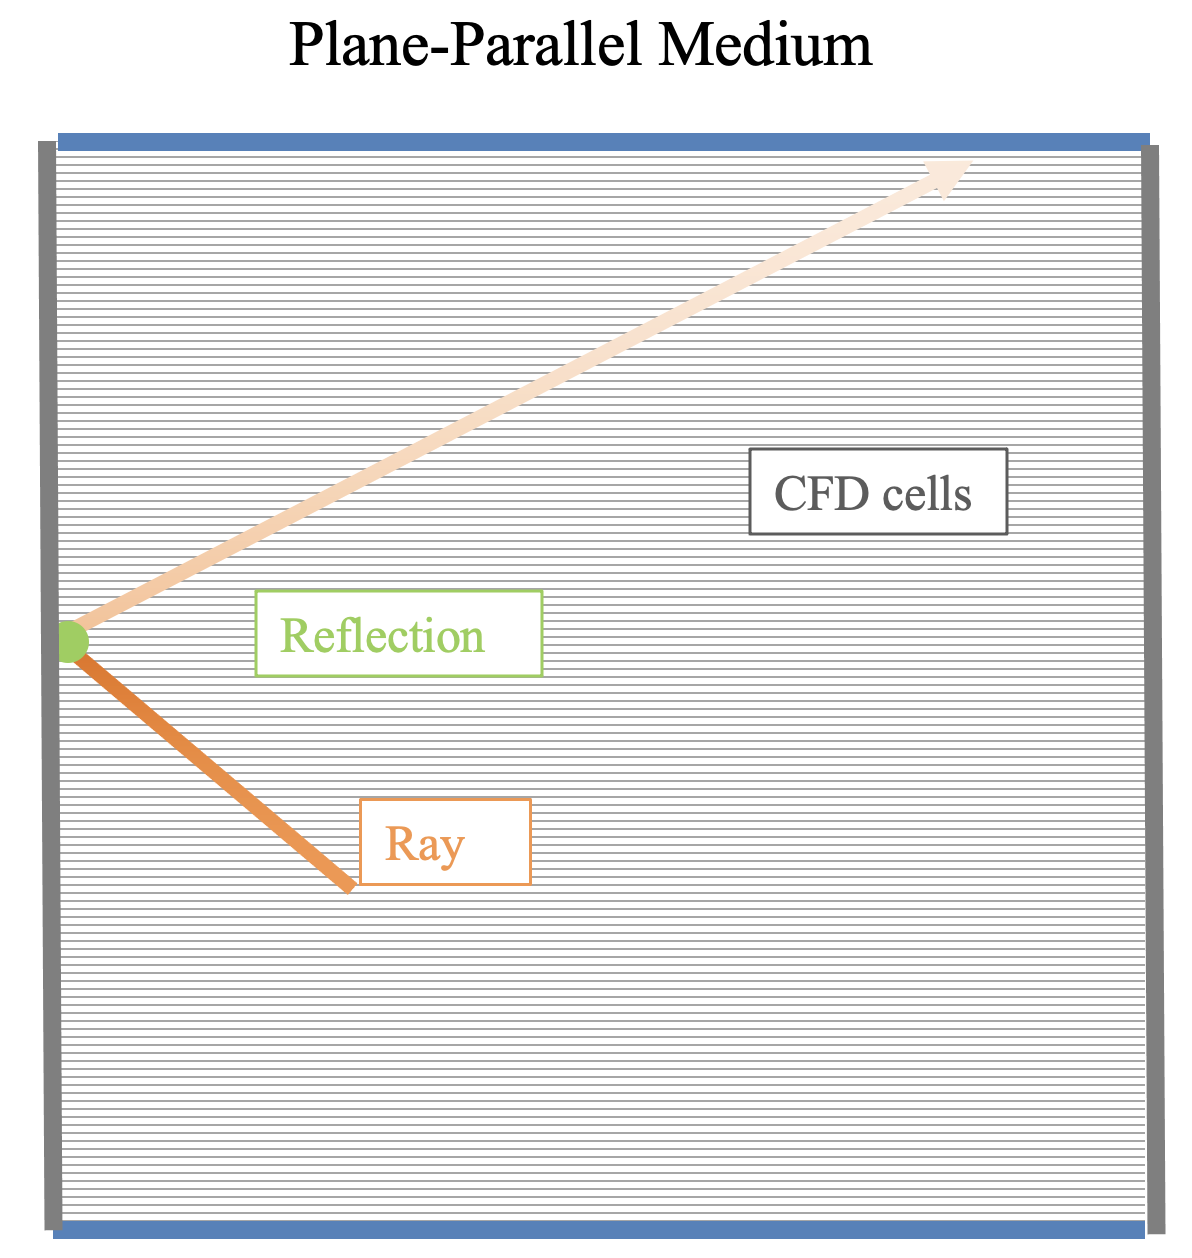
\includegraphics[width=0.5\linewidth]{figures/ch4/PlaneParallel.png}
\caption{A one-dimensional plane parallel medium. Red walls are symmetric and blue walls are cold and black. Ray is in orange.}
\label{fig:PlaneParallel2}
\end{figure}

\subsection{Results for a single MPI rank}
The various tracing methods are first tested within a single MPI-rank on a single computing node.
Figures~\ref{fig:PPcomp_kappa} to \ref{fig:PPcomp_temp} display comparisons of the volumetric radiative absorption of the mean MCRT results alongside the exact solutions.
Results show excellent agreement under all absorption coefficients and temperatures. 
\begin{figure}[!ht]
\centering
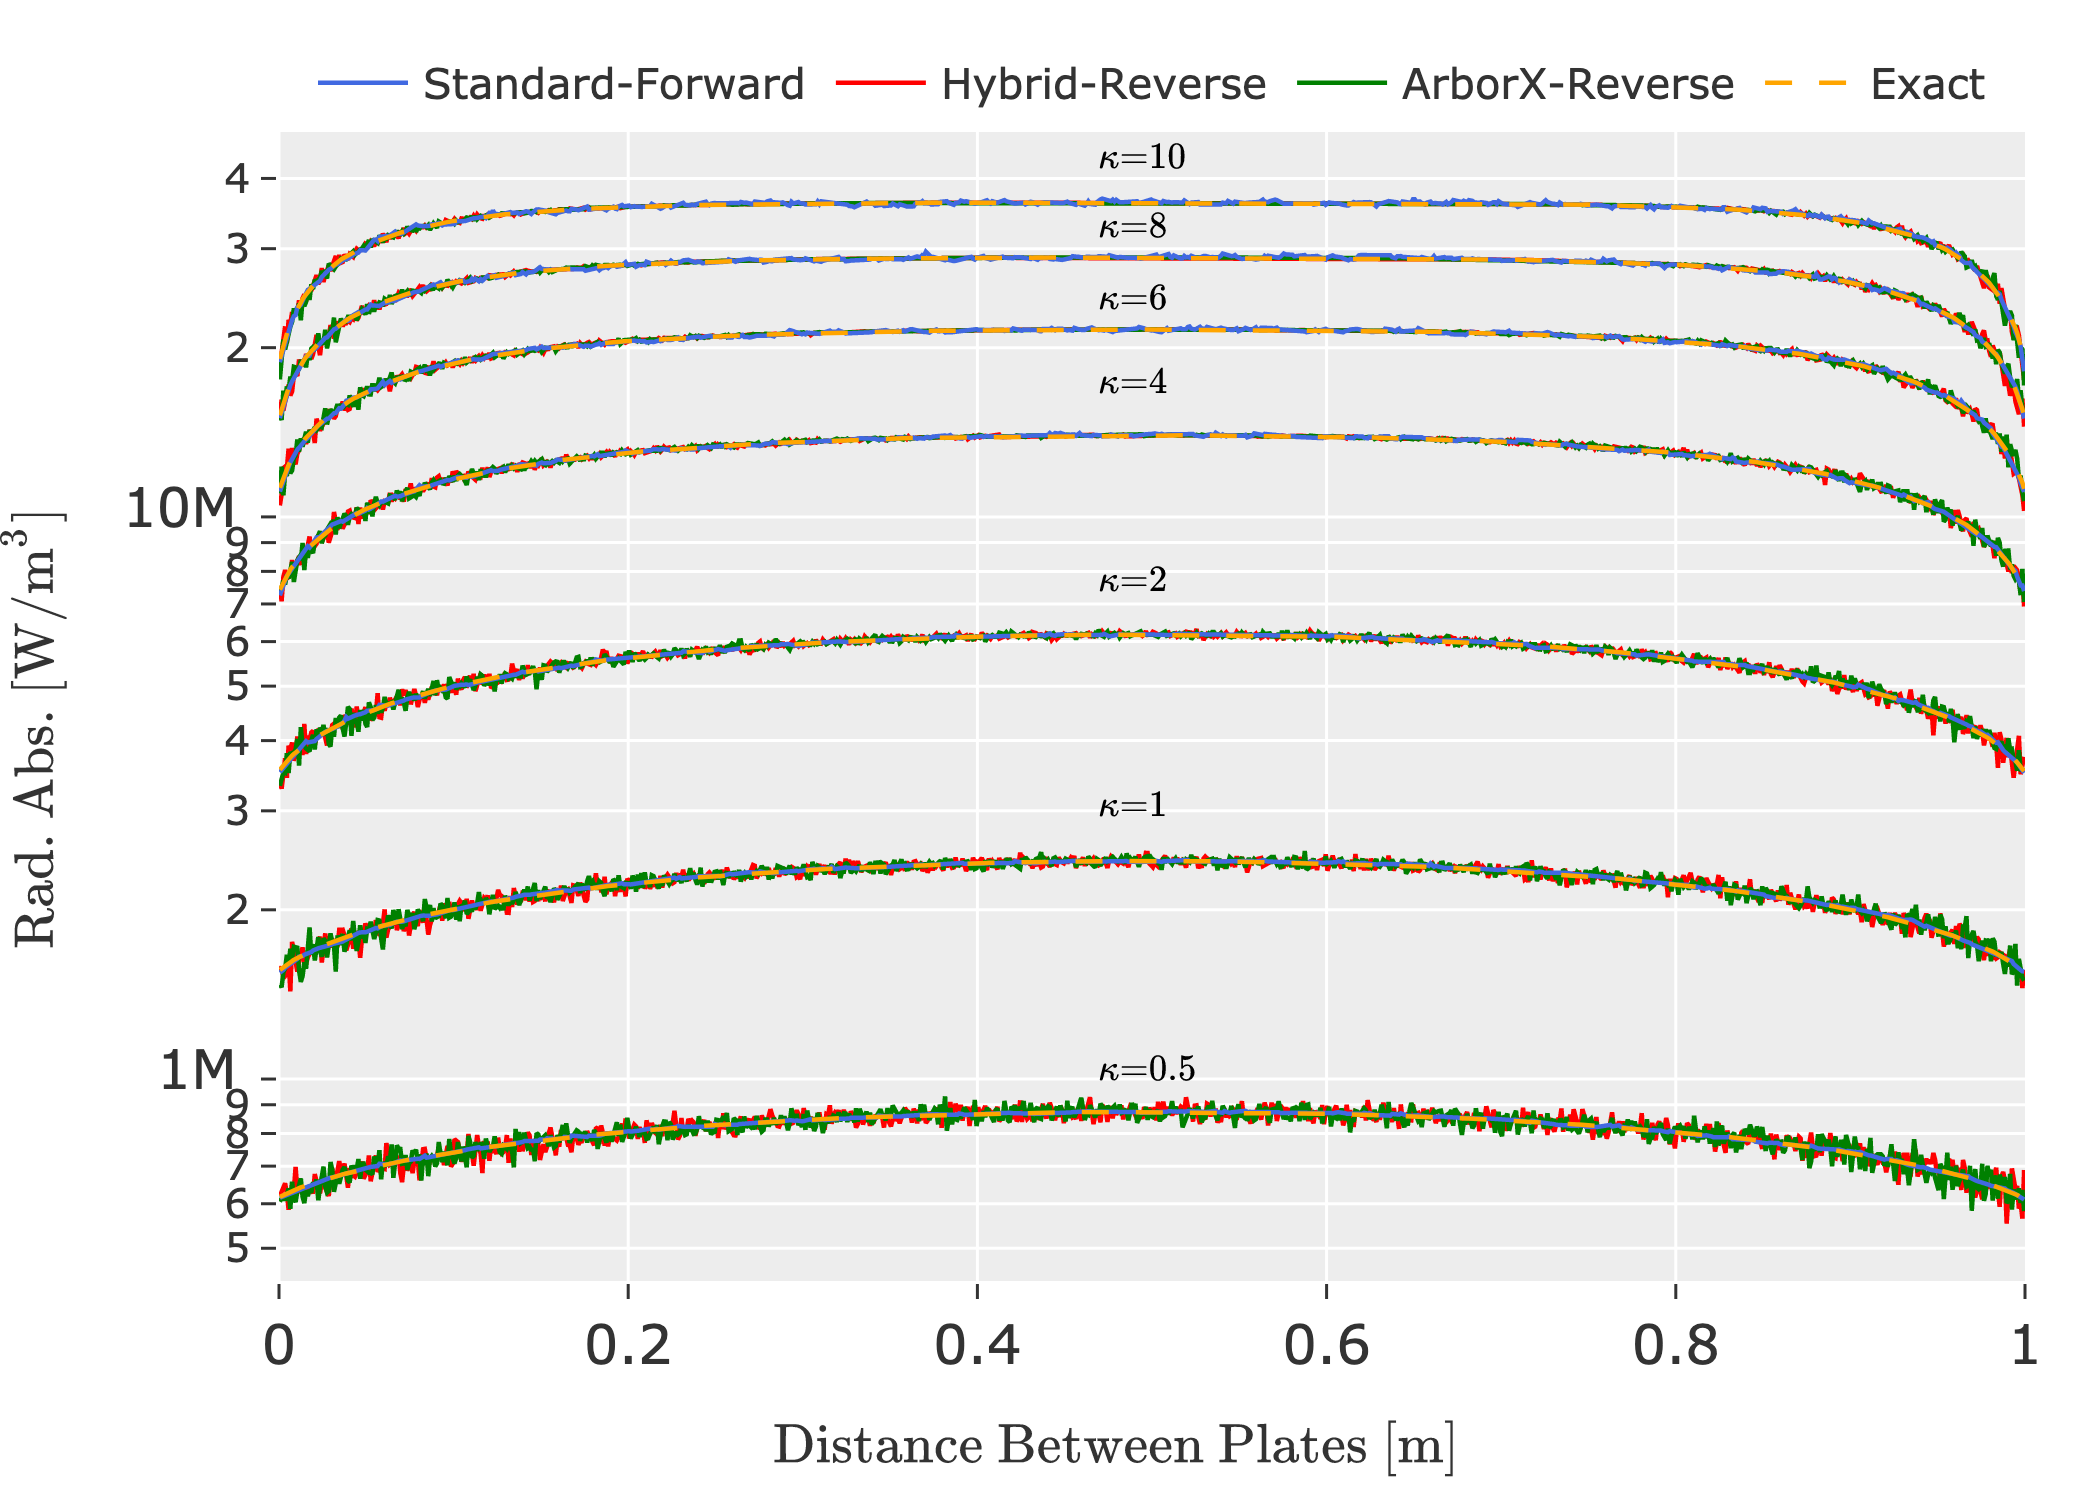
\includegraphics[width=0.95\linewidth]{figures/ch4/PPcomparison1.png}
\caption{Comparison of the absorption source term using variable absorption coefficient $\kappa{}$ in m$^{-1}$ with T=$2000$K, N$_r$=$1000$, N$_{cells}$=1000 on a single MPI rank.}
\label{fig:PPcomp_kappa}
\end{figure}
\begin{figure}[!ht]
\centering
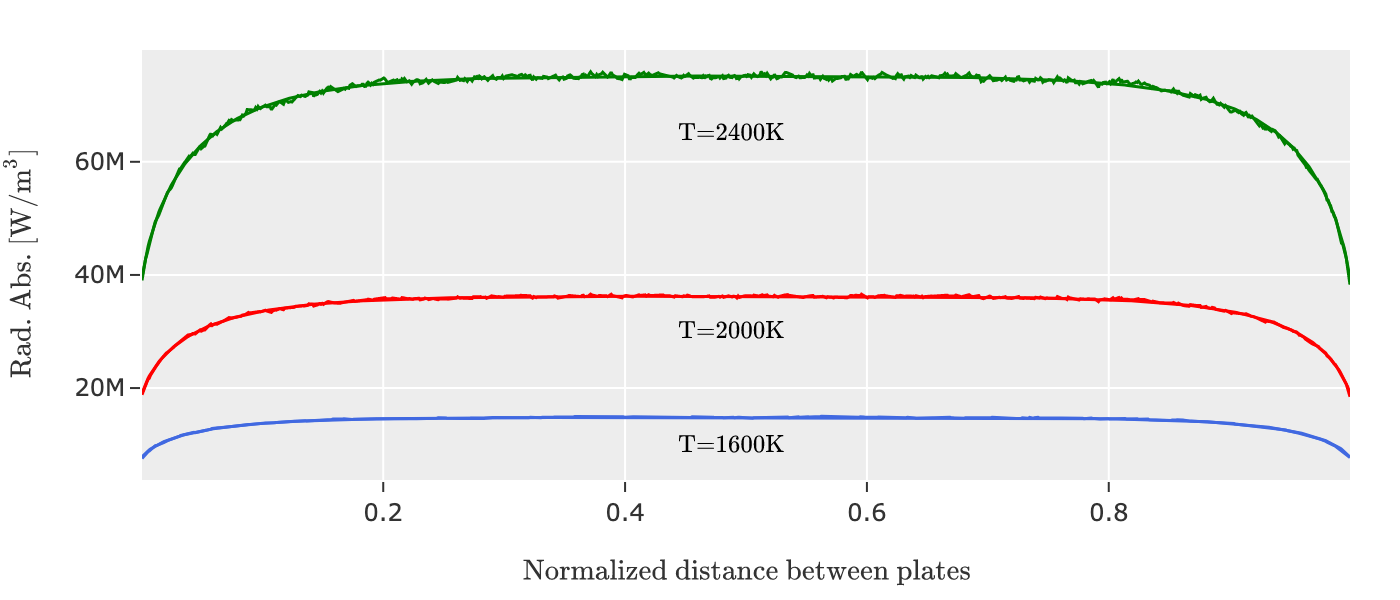
\includegraphics[width=0.95\linewidth]{figures/ch4/PPcomparison2.png}
\caption{Variable temperature with $\kappa{}$=$10$ m$^{-1}$, N$_r$=$1000$, N$_{cells}$=1000 on a single MPI rank.}
\label{fig:PPcomp_temp}
\end{figure}


Tables~\ref{table:PPcomp_std} and~\ref{table:PPcomp_temp} list the maximum standard deviations normalized by the average of all radiative absorptions for all computational cells and runs at each each condition. Normalized standard deviations $\sigma_{max,norm}$ are evaluated using the method described in Ref.~\cite{Modest2022ChapterExchange}, as 
\begin{equation}
    \sigma(x) = \sqrt{\frac{\sum_i^{N_s}{(Q_{abs,MCRT,i}(x)-\overline{Q_{abs,MCRT,i}(x)})^2}}{N_s(N_s-1)}}~\text{, and}
    \label{eq:StandardDeviation}
\end{equation}
\begin{equation}
    \sigma_{max,norm} = \frac{\text{max}_x(\sigma(x))}{\widetilde{Q_{abs,MCRT}}}~,
    \label{eq:StandardDeviationMax}
\end{equation}
where $i$ is one of $N_s$ samples, $x$ is the distance between the plates, and $\bar{~}$ and $\widetilde{~}$ indicate averages over the $50$ sampled runs and over all radiative absorptions, respectively. 
Tables~\ref{table:PPcomp_std} and \ref{table:PPcomp_temp} again show good agreement with analytical solutions, with maximum normalized standard deviations of less than 5\%.

In the reverse methods, a noticeable degree of noise is present near the boundaries of the medium. This is a natural occurrence in the reverse Monte Carlo method~\cite{Farmer1998ComparisonMedia}. Reverse rays emitted from the center of the medium encounter identical medium composition on all sides and for approximately the same lengths. As a result, cells in this region observe minimal variance in accumulated intensities. However, near the edges, a large fraction of the rays reach the boundary instead of the medium. These rays return different intensities from those directed into the medium, resulting in an increased variance in absorption.
This trend occurs in increasing magnitude for lower absorption coefficients~\cite{Farmer1998ComparisonMedia}. As absorption coefficient decreases, the optical distance from the center of the medium to the boundaries decreases; subsequently, decreasing absorption coefficient increases the variance towards the center of the medium. Figure~\ref{fig:PPcomp_kappa} demonstrates these trends with significant magnification due to the logarithmic axis visually inflating errors for low-absorption coefficient runs.



\begin{table}
\centering
\caption{Maximum normalized standard deviations (using Eq.~\ref{eq:StandardDeviationMax}) for various MCRT results at various absorption coefficients.}
\begin{tabular}{c c c c c c c c} 
\hline
\multirow{ 2}{*}{\bfseries Tracing Method} & 
\multicolumn{7}{c}{\bfseries Abs. Coeffs. [m$^{-1}$]} \\ [0.5ex] \cline{2-8}
 & $0.5$ & $1$ & $2$ & $4$ & $6$ & $8$ & $10$\\ [0.5ex]
 \hline
 Standard-Forward & $0.0079$ & $0.0084$ & $0.0068$ & $0.0074$ & $0.0079$ & $0.0088$ & $0.0095$\\ [0.5ex] 
 ArborX-Reverse & $0.046$ & $0.038$ & $0.032$ & $0.027$ & $0.026$ & $0.024$ & $0.025$\\ [0.5ex] 
 Hybrid-Reverse & $0.046$ & $0.038$ & $0.030$ & $0.028$ & $0.027$ & $0.026$ & $0.024$\\ [0.5ex] 
 % $\overline{Q_{abs,MCRT}}$ & $804313.45$ & $2210805.26$ & $34486563.86$ & $5551660.80$ & $12715801.18$ & $19956132.77$ & $27212767.06$ \\
 \hline
\end{tabular}
\label{table:PPcomp_std}
\end{table}

Figures~\ref{fig:PPcomp_kappa} also demonstrates the physical result of increasing absorption coefficient to the reader. It is apparent that higher absorption coefficients result in higher volumetric radiative absorption within the medium. 
This is evident from Beer's law, Eq.~\ref{eq:BeersLaw}, which shows how increasing absorption coefficient results in an increase in attenuation of ray intensity.
Furthermore, higher absorption coefficients increase the radiative emission as well, per Eq.~\ref{eq:emitting_sphere}. This increases the amount of energy available to be absorbed. The net effect is a super-linear increase in radiative absorption. Between absorption coefficients of $1~m^{-1}$ and $2~m^{-1}$, for example, peak radiative absorption increases almost three times.

Regarding the shape of the absorption profiles, towards the center of the media, larger absorption is apparent due to a higher amount of incident radiation from the emitting medium on both sides.
Towards the edges, radiative absorption decreases due to the absence of radiation from the adjacent cold-black wall. Additionally, high absorption coefficients result in a flattened radiative absorption profile. This again follows from the exponential nature of Beer's law. As absorption coefficient increases, rays are attenuated more rapidly by the medium, allowing less energy to escape to the wall.

\begin{table}
\centering
\caption{Maximum normalized standard deviations (using Eq.~\ref{eq:StandardDeviationMax}) for various MCRT results at various temperatures.}
\begin{tabular}{c c c c} 
\hline
\multirow{ 2}{*}{\bfseries Tracing Method} & 
\multicolumn{3}{c}{\bfseries Temperatures [K]} \\ [0.5ex] \cline{2-4}
 & $1600$ & $2000$ & $2400$ \\ [0.5ex]
 \hline
 Standard-Forward & $0.0097$ & $0.0091$ & $0.0091$ \\ [0.5ex] 
 ArborX-Reverse & $0.025$ & $0.025$ & $0.026$ \\ [0.5ex] 
 Hybrid-Reverse & $0.025$ & $0.024$ & $0.024$ \\ [0.5ex] 
 % $\overline{Q_{abs,MCRT}}$ & $804313.45$ & $2210805.26$ & $34486563.86$ & $5551660.80$ & $12715801.18$ & $19956132.77$ & $27212767.06$ \\
 \hline
\end{tabular}
\label{table:PPcomp_temp}
\end{table}

Likewise, when temperature is increased, as shown in Fig.~\ref{fig:PPcomp_temp}, radiative absorption also increases. This follows from the increased emission due to the fourth order scaling of temperature in the black-body emission function, Eq. \ref{eq:PlancksLaw}.
An increase in temperature of $400$K approximately doubles the net radiation absorbed.



\begin{table}
\centering
\caption{Average runtimes for each tracing method.}
\begin{tabular}{c c c c} 
\hline
 & Standard-Forward & ArborX-Reverse & Hybrid-Reverse \\ [0.5ex]
 \hline
 Runtime (s) & $0.048$ & $0.074$ & $0.052$ \\ [0.5ex] 
 \hline
\end{tabular}
\label{table:PP_runtimes}
\end{table}

Solver runtimes are presented in Table~\ref{table:PP_runtimes}. All solutions are conducted using Intel Xeon Gold 5220 processors using the Kokkos OpenMP back-end with 72 OpenMP threads. Runtimes appeared to be independent of absorption coefficient and temperature with the exception of the Standard-Forward method where rays are terminated in the mesh when they fall below a cutoff energy. As a result, Standard-Forward saw decreasing runtime with increasing absorption coefficient. As such, presented runtimes are averaged across all cases tested except for Standard-Forward where the maximum runtime is presented. Standard-Forward is noticeably faster than ArborX-Reverse. This is likely a result of the BVH tracing procedure. For ArborX-Reverse, the BVH must be traversed once for every ray to determine the intersected cells. A BVH traversal requires more time to compute than the standard computation of determining the next cell intersected by using the exit face of the previous cell. As a result, ArborX-Reverse requires more time to simulate within a single MPI rank. Hybrid-Reverse, however, requires a similar runtime as both Hybrid-Reverse and Standard-Forward conduct identical tracing operations when run within one MPI rank. Hybrid-Reverse, however, requires rays to propagate until exiting the domain instead of terminating upon falling below a cutoff energy. Therefore, Hybrid-Reverse does not see the trend of decreasing runtime with increasing absorption coefficient.

\begin{figure}[!ht]
\centering
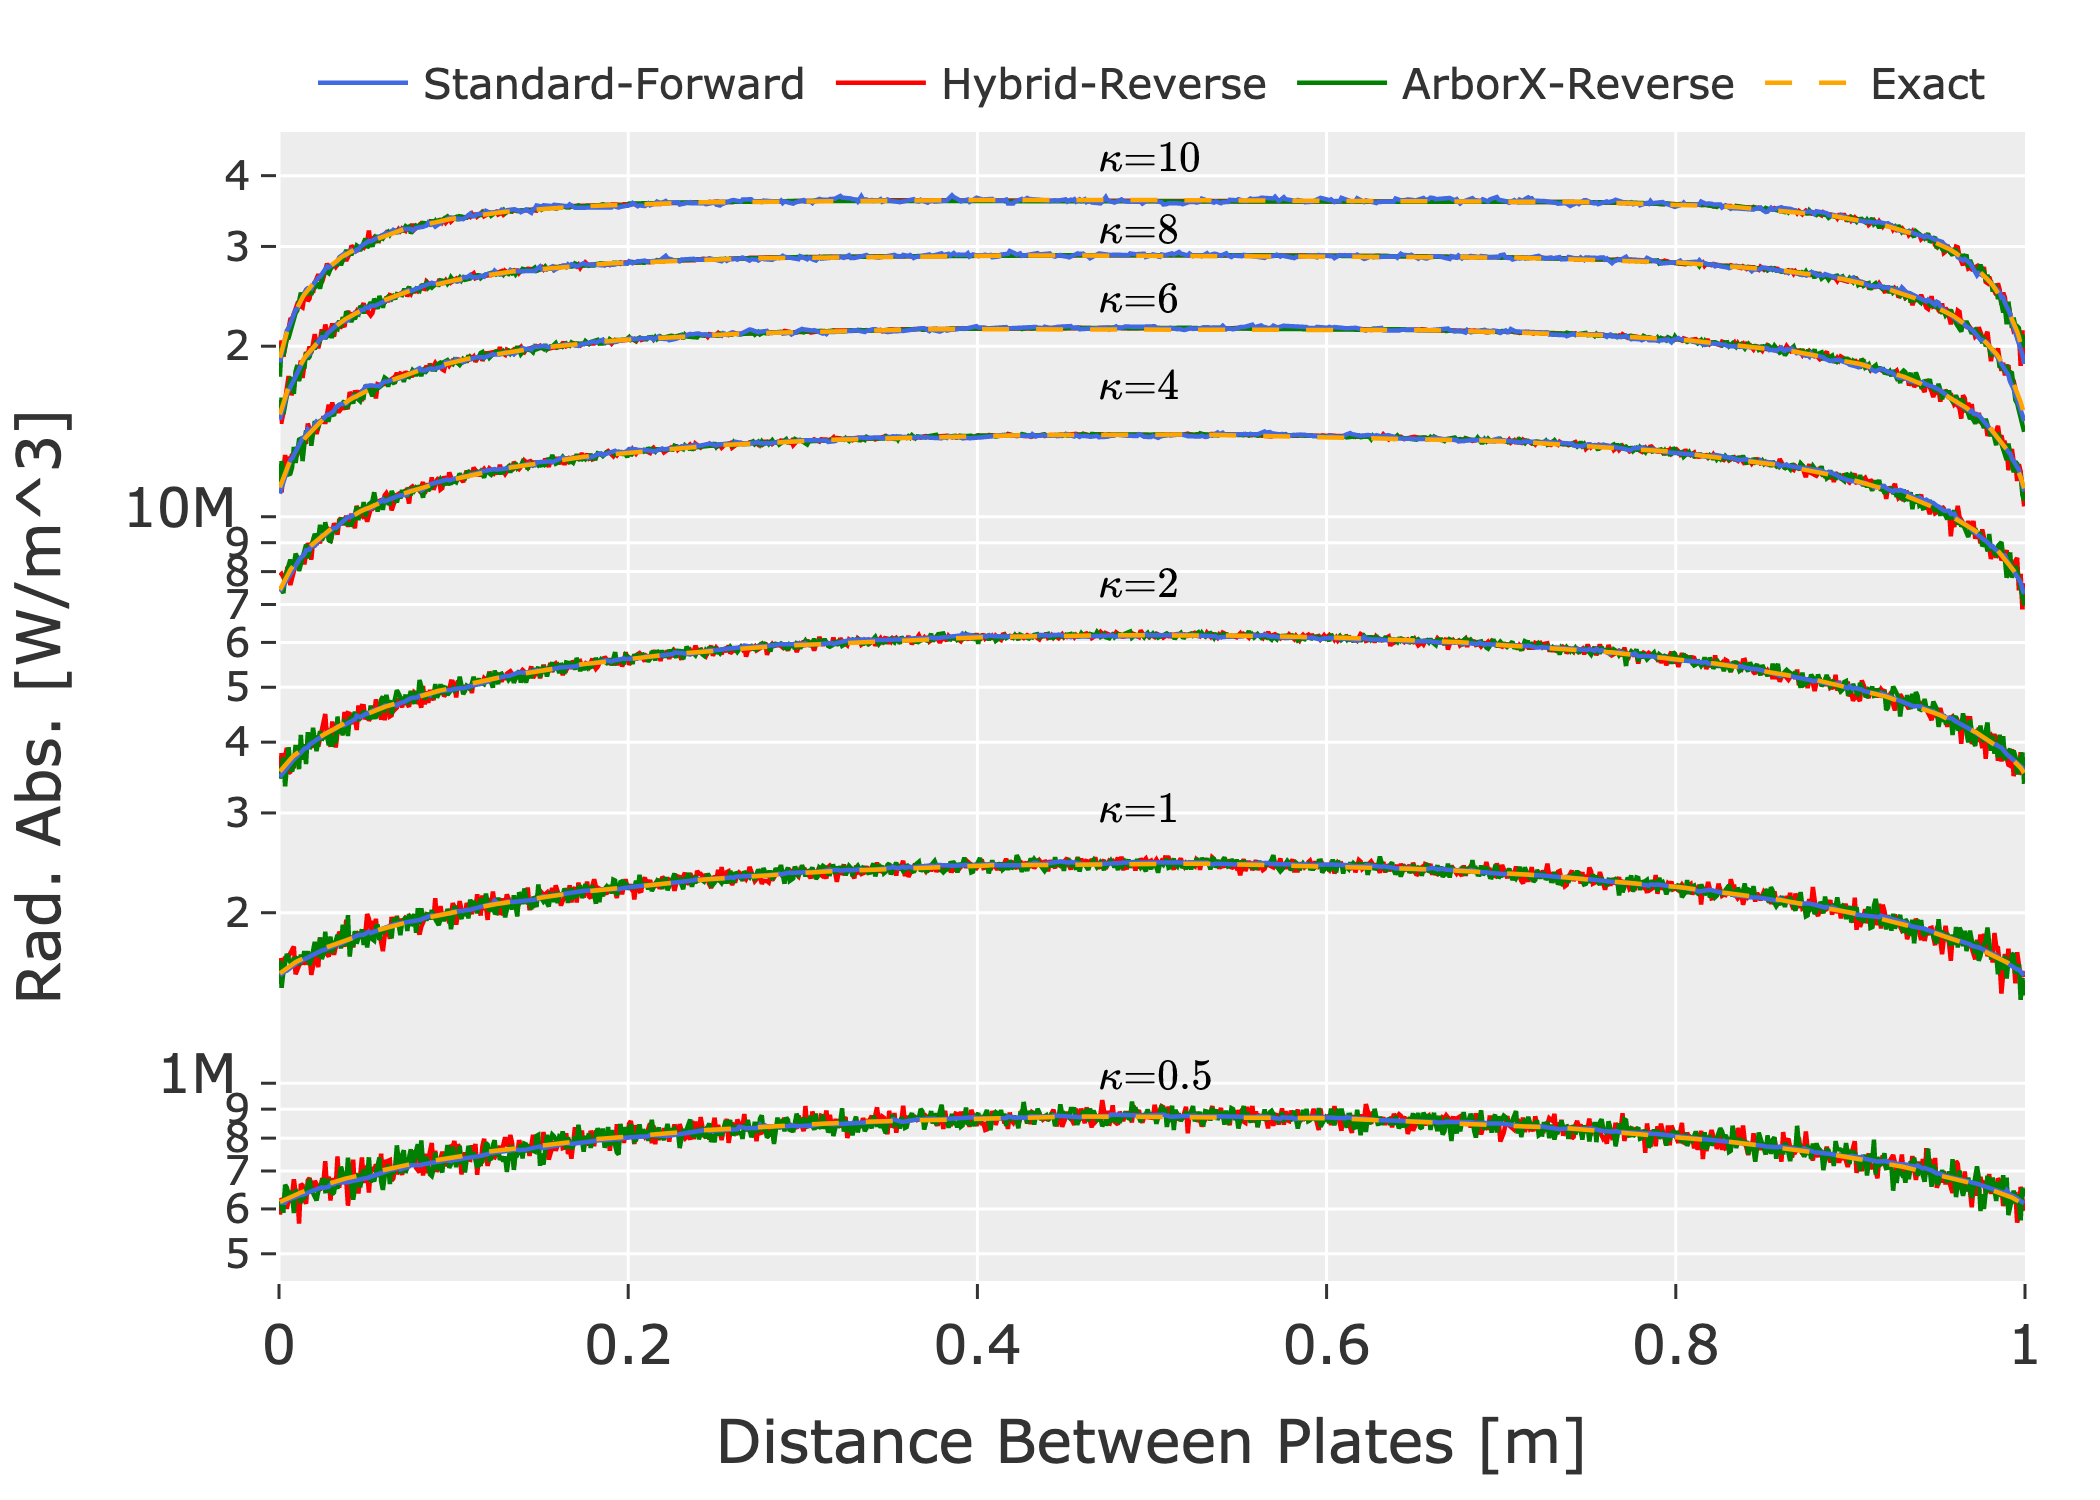
\includegraphics[width=0.95\linewidth]{figures/ch4/PPcomparison1_multinode.png}
\caption{Variable absorption coefficient $\kappa{}$ in m$^{-1}$ with T=$2000$K, N$_r$=$1000$, N$_{cells}$=1000 with eight MPI ranks.}
\label{fig:PPcomp_kappa_mpi}
\end{figure}
\begin{figure}[!ht]
\centering
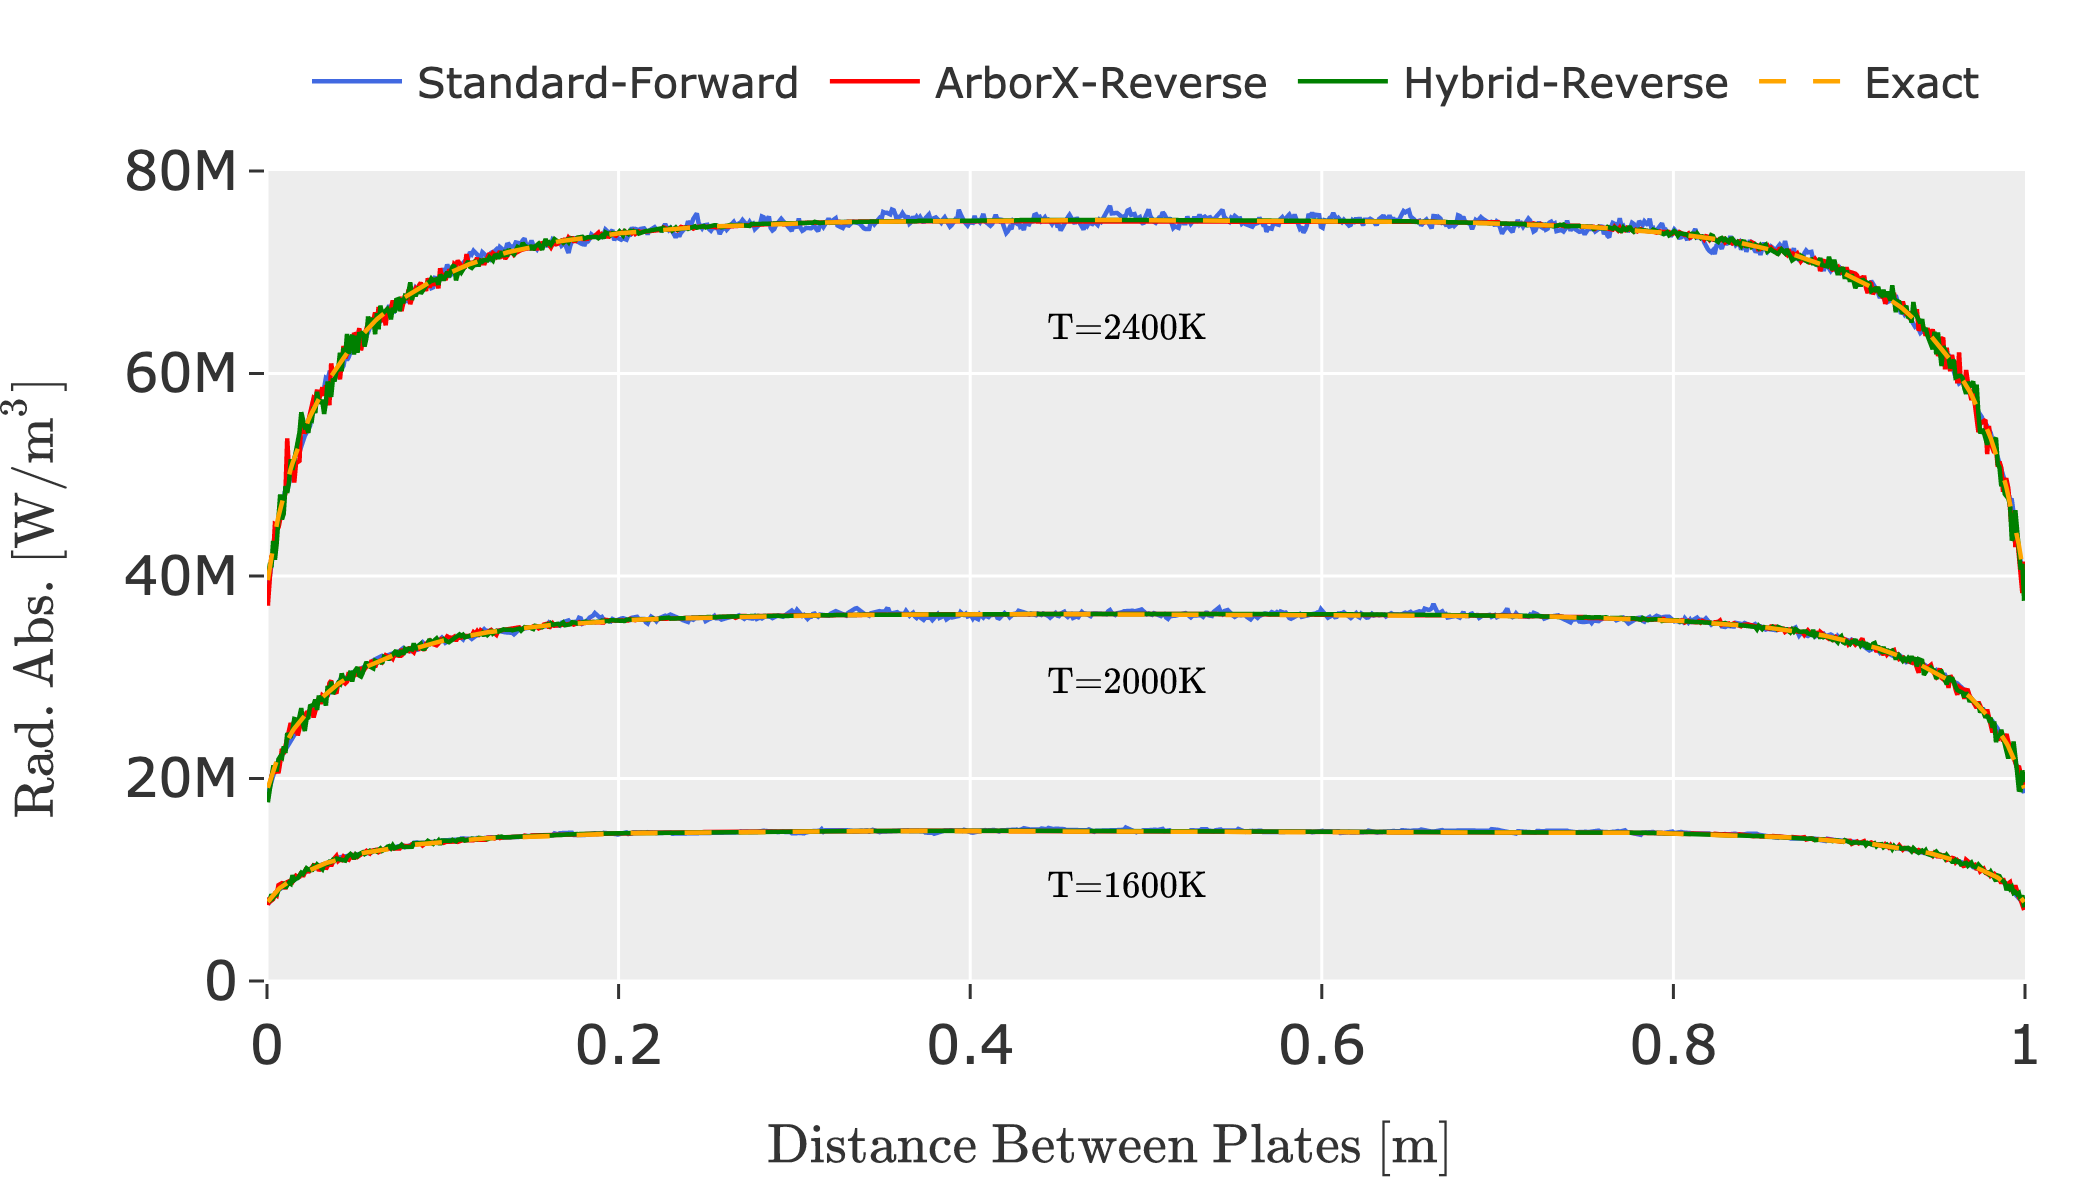
\includegraphics[width=0.95\linewidth]{figures/ch4/PPcomparison2_multinode.png}
\caption{Variable temperature with $\kappa{}$=$10$ m$^{-1}$, N$_r$=$1000$, N$_{cells}$=1000 with eight MPI ranks.}
\label{fig:PPcomp_temp_mpi}
\end{figure}
\subsection{Results with multiple MPI ranks}
The same tracing procedures are tested on the same plane-parallel configuration with eight MPI ranks evenly spaced along the one-dimensional domain.
Monte Carlo and exact solutions are compared at varying absorption coefficients and temperatures and results are presented in Figs.~\ref{fig:PPcomp_kappa_mpi} and~\ref{fig:PPcomp_temp_mpi}. As before, results compare extremely well demonstrating the accuracy of the distributed raytracing method of section~\ref{section:MPIacceleration}. Similar to the single-node results, an increase of solution noise is observed for the reverse Monte Carlo solutions at lower absorption coefficients due to the boundary effect discussed previously. Tables~\ref{table:PPcomp_std_mpi} and \ref{table:PPcomp_temp_mpi} display maximum normalized standard deviations for all MPI runs. As before, standard deviations are greater in the reverse Monte Carlo results than in the Standard-Forward results. Finally, overall-averaged runtimes are presented in Table~\ref{table:PP_runtimes_mpi} for each of the solvers. For these results, ArborX-Reverse exhibits greater performance compared to Standard-Forward and Hybrid-Reverse. 



\begin{table}
\centering
\caption{Maximum normalized standard deviations (using Eq.~\ref{eq:StandardDeviationMax}) for various MCRT results at various absorption coefficients for with eight MPI-ranks.}
\begin{tabular}{c c c c c c c c} 
\hline
\multirow{ 2}{*}{\bfseries Tracing Method} & 
\multicolumn{7}{c}{\bfseries Abs. Coeffs. [m$^{-1}$]} \\ [0.5ex] \cline{2-8}
 & $0.5$ & $1$ & $2$ & $4$ & $6$ & $8$ & $10$\\ [0.5ex]
 \hline
 Standard-Forward & $0.0090$ & $0.0066$ & $0.0067$ & $0.0070$ & $0.0085$ & $0.0089$ & $0.0096$\\ [0.5ex] 
 ArborX-Reverse & $0.0439$ & $0.0375$ & $0.0348$ & $0.0306$ & $0.0309$ & $0.0265$ & $0.0239$\\ [0.5ex] 
 Hybrid-Reverse & $0.0439$ & $0.0381$ & $0.0345$ & $0.0290$ & $0.0262$ & $0.0248$ & $0.0231$\\ [0.5ex] 
 \hline
\end{tabular}
\label{table:PPcomp_std_mpi}
\end{table}


\begin{table}
\centering
\caption{Maximum normalized standard deviations (using Eq.~\ref{eq:StandardDeviationMax}) for various MCRT results at various temperatures with eight MPI ranks.}
\begin{tabular}{c c c c} 
\hline
\multirow{ 2}{*}{\bfseries Tracing Method} & 
\multicolumn{3}{c}{\bfseries Temperatures [K]} \\ [0.5ex] \cline{2-4}
 & $1600$ & $2000$ & $2400$ \\ [0.5ex]
 \hline
 Standard-Forward & $0.0097$ & $0.0091$ & $0.0091$ \\ [0.5ex] 
 ArborX-Reverse & $0.025$ & $0.025$ & $0.026$ \\ [0.5ex] 
 Hybrid-Reverse & $0.025$ & $0.024$ & $0.024$ \\ [0.5ex] 
 \hline
\end{tabular}
\label{table:PPcomp_temp_mpi}
\end{table}

\begin{table}
\centering
\caption{Average runtimes for each tracing method.}
\begin{tabular}{c c c c} 
\hline
 & Standard-Forward & ArborX-Reverse & Hybrid-Reverse \\ [0.5ex]
 \hline
 Runtime (s) & $1.25$ & $1.10$ & $1.21$ \\ [0.5ex] 
 \hline
\end{tabular}
\label{table:PP_runtimes_mpi}
\end{table}



\subsection{Results with varying ray counts}
Finally, Fig.~\ref{fig:PPcom_nrays} presents the radiative absorption profile for different ray counts. Only Standard-Forward results are presented in this figure to demonstrate the general effect of ray count on solution variance. Absorption coefficients and temperatures are held constant at $10~m^{-1}$ and $2000$ K.
Increasing ray counts result in decrease of stochastic noise in the solution. Table \ref{table:PPcomp_rayct} displays maximum standard deviations for each of the three tests. As the number of rays increases, the variability decreases and the solution approaches the exact. As per \citet{Modest2022ChapterExchange}, the standard deviation should be proportional to $1/N_r^{1/2}$ for $N_r$ rays. This would mean an increase of ray count by one order of magnitude should decrease standard deviation by a factor of $\frac{1}{\sqrt{10}} = 0.32$. Table~\ref{table:PPcomp_rayct} shows that this trend is closely followed by showing the ratio of the maximum standard deviation of higher ray counts to that of lower ray counts.


\begin{table}
\centering
\caption{Standard deviations of the percent difference of MCRT and exact solution at various absorption coefficients. Each simulation is run with $1000$ computational cells, a temperature of $2000$K, and absorption coefficient of 10m$^{-1}$}.
\begin{tabular}{c c c c} 
 \hline
 Rays emitted per cell & $10$ & $100$ & $1000$ \\ [0.5ex] 
 \hline
 Eq.~\ref{eq:StandardDeviationMax} & $4.83$ & $1.47$ & $0.52$ \\
 Ratio of standard deviations & ~ & $\frac{1.47}{4.83}=0.30$ & $\frac{0.52}{1.47}=0.35$ \\
 \hline
\end{tabular}
\label{table:PPcomp_rayct}
\end{table}
\begin{figure}
\centering
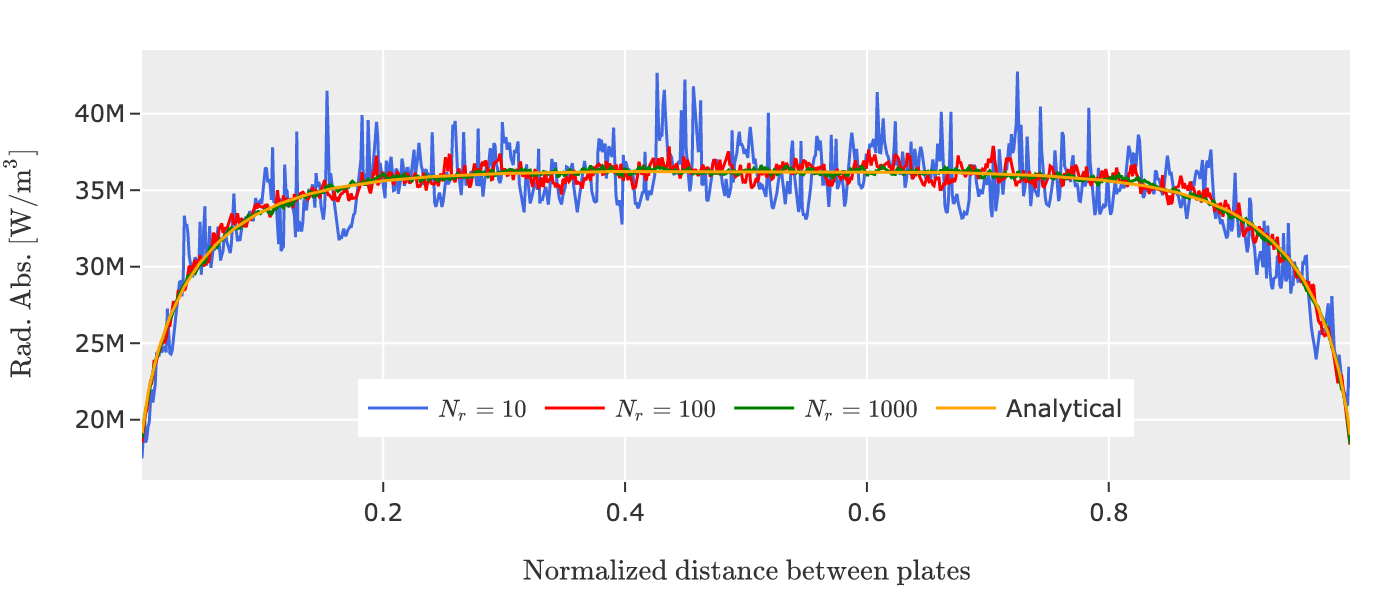
\includegraphics[width=0.95\linewidth]{figures/ch4/PPcomparison3.png}
\caption{Variable number of rays emitted per cell (N$_r$) with $\kappa{}$=$10$ m$^{-1}$, T=$2000$K, N$_{cells}$=1000.}
\label{fig:PPcom_nrays}
\end{figure}
% \subsection{Profiling}



% The lower variance, however, comes at the expense of additional runtime. 

% Profiling results from the plane-parallel medium were then 

% \begin{figure}



%   \label{fig:PPcomp}
% \end{figure}



\section{Backward-Facing Step Combustor}\label{section:BFS}
The backward-facing step (BFS) combustor is another simple, repeatable geometry that is used for a variety of case studies in fluid dynamics. 
The BFS geometry is presented in Fig.~\ref{fig:BFS_geometry} and is based on an experimental configuration at the Pennsylvania State University.
Fluid enters through the inlet and flows over the step towards the outlet. When the gas moves past the step, it forms a large a recirculation zone, which mimics similar fluid dynamic phenomenon within a real combustor. 

The interaction between the fluid and the boundaries, the characteristics of turbulent fluctuations, and the resulting mean velocities profiles are all topics of interest when studying backward-facing steps. 
Numerous examples exist demonstrating its use for experimental and numerical investigations of turbulent fluid flow~\cite{Armaly1983ExperimentalFlow,Neto1993AStep,Jovic1994Backward-facing5000,Le1997DirectStep}. 
Most computational studies in literature are conducted with non-reacting, isothermal conditions.
In contrast, studies of combined turbulent and high temperature flow~\cite{Niemann2016Buoyancy-affectedNumber,Xie2017GeometrySteps}, and reacting flows~\cite{Pouech2021PremixedStep} over backward-facing steps have been modeled significantly less frequently.
In the relatively few studies that exist, the addition of volumetric heating and composition changes resulting from the exothermic chemical reactions have been shown to influence the flow patterns and turbulence intensity of the fluid~\cite{Pouech2021PremixedStep}. 

Recent work related to the present radiation solver has focused on quantifying the relative contribution of radiative to convective heat transfer on the boundaries of reacting backward-facing step systems~\cite{Colborn2023VariationCombustor}.
To that end, a combined experimental and modeling collaboration is underway between the Pennsylvania State University and the University of Connecticut to study this. In the future, results from the Penn-State experimental rig will be compared to computational results obtained using the present radiation solver to better understand the heat transfer mechanism. For this thesis, the same geometry is used to demonstrate the accuracy and efficiency of the radiation solver within a research-relevant geometry.

First, a description of the case setup is provided. Next, results from the Standard-Forward implementation are compared against those of an established Fortran code. Results are obtained using the Standard-Forward solver because it is the most robust solver at the present stage of development.
% ArborX-Reverse and Hybrid-Reverse also exhibited increased variance present in the previous section. 
Then, a description of the influences of radiation in the fluid and along the walls is provided. Finally, solver runtimes are presented and compared.



\subsection{Case setup}

\begin{figure}
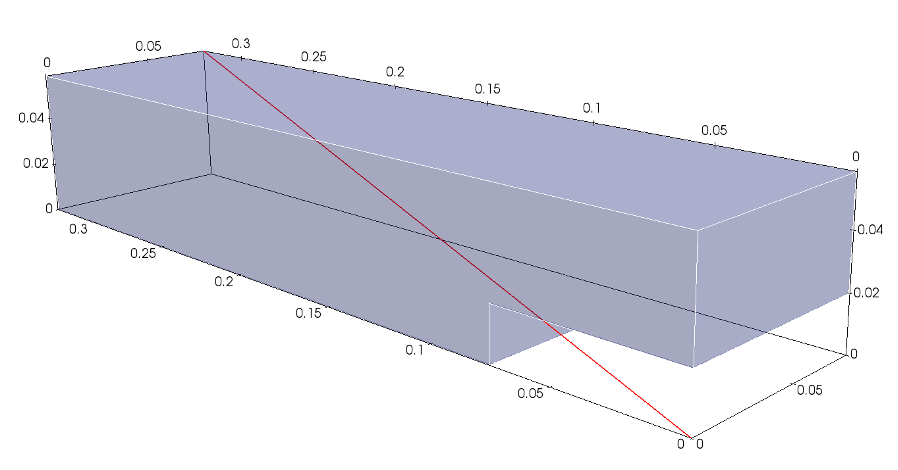
\includegraphics[width=\linewidth]{figures/ch4/BFS_geometry.png}
\caption{Dimensions of backward-facing step configuration used in this study in addition to a representative line used to sample radiative properties. The sampled line connects the farthest two corners of the bounding box around the domain.}
\label{fig:BFS_geometry}
\end{figure}

The simulation domain is identical to that of a previous study~\cite{Toumey2021DevelopmentTransfer}. The geometry is $33$ centimeters long between the inlet and the outlet and $8$ centimeters in width. The mesh consists of $7,411,200$ hexahedral cells of increasing refinement at the recirculation zone and the walls.
For this case, no chemically reacting flow is included. 
The flow is present in vitiated form, where a chemical reaction is initiated in a region upstream of the step, and the resulting "dirty" air with high CO$_2$ and H$_2$O content is diluted with quiescent air before entering the domain. All subsequent chemical reactions are neglected beyond the simulation inlet, resulting in a purely fluid-mechanic and heat-transfer calculation within the simulation domain. Furthermore, the present simulation does not contain any chemical composition data, so accurate absorption coefficients cannot be calculated. Therefore, the absorption coefficient is assumed to be a uniform value of 0.5~m$^{-1}$.
The mixture reaches the main section at a temperature of up to $850$K, appreciably lower than expected temperatures of above $1600$K when full reactions are present. Pressure is atmospheric, and inlet velocities are approximately $10$ m/s.
The simulations are conducted using the conjugate heat transfer solver \texttt{multiRegionReactingFoam}, which is a compressible solver that accounts for energy transport. The region boundaries are all treated as cold, black boundaries with the exception of the sidewalls that are treated as symmetric planes.



\subsection{Results}
A single time-step of the CFD simulation after 1.094 seconds of physical time was extracted for a frozen field analysis. Ten rays are emitted for each computational cell.
Figures \ref{fig:BFS_temperature}, \ref{fig:BFS_streamlines} show temperature contours and velocity streamlines at the frozen timestep in the simulation. The vitiated flow is shown to partially whirl downward and recirculate behind the step. At this point, the mostly laminar entry gas quickly becomes turbulent and chaotic.

\begin{figure}
  \begin{subfigure}{1\textwidth}
  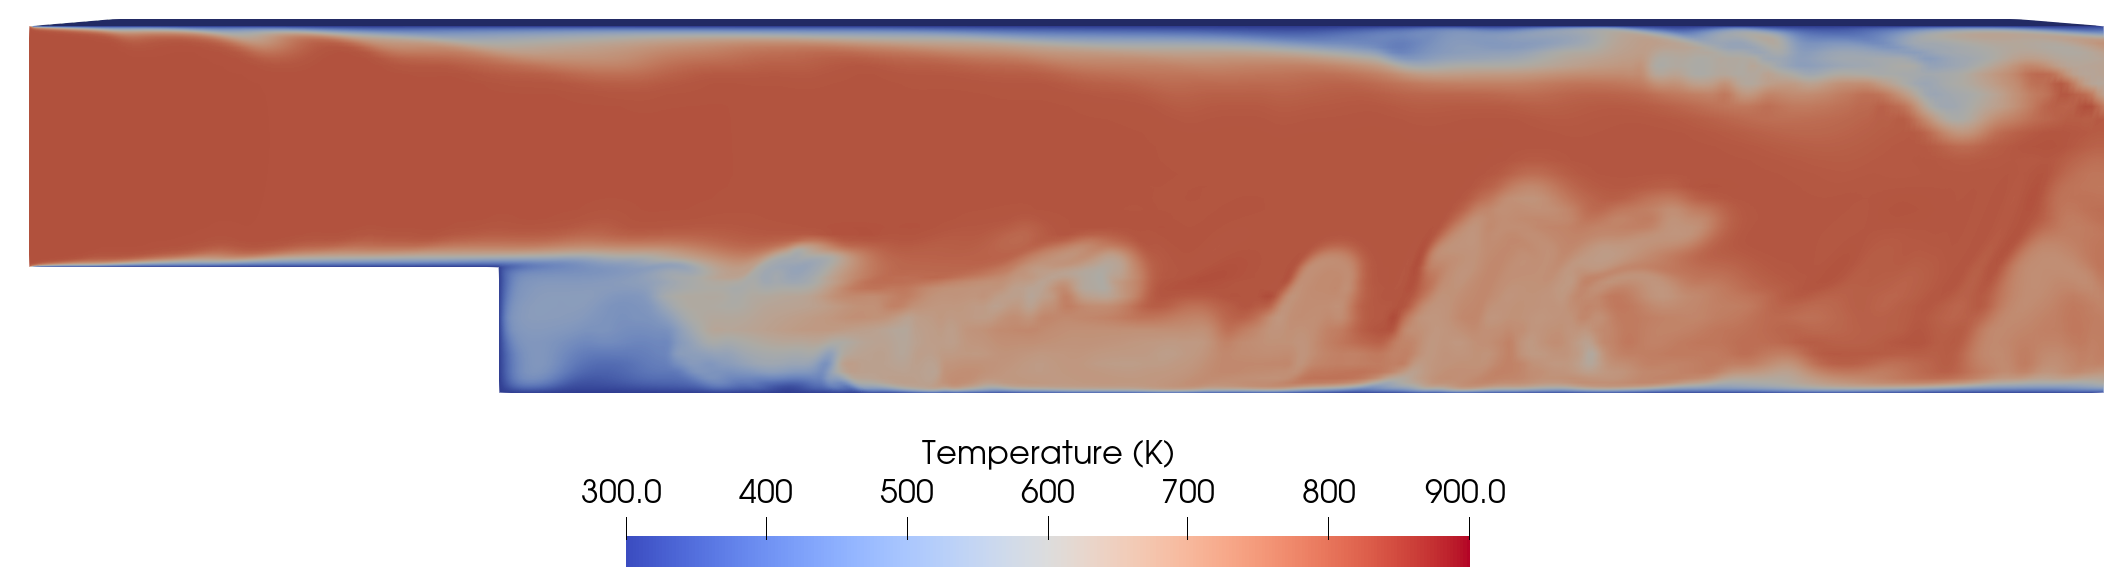
\includegraphics[width=\linewidth]{figures/ch4/BFS_temperature.png}
  \caption{BFS temperature contour along the mid-plane after $1.094$ seconds of physical time in the simulation. }
  \label{fig:BFS_temperature}
  \end{subfigure}
  \begin{subfigure}{1\textwidth}
  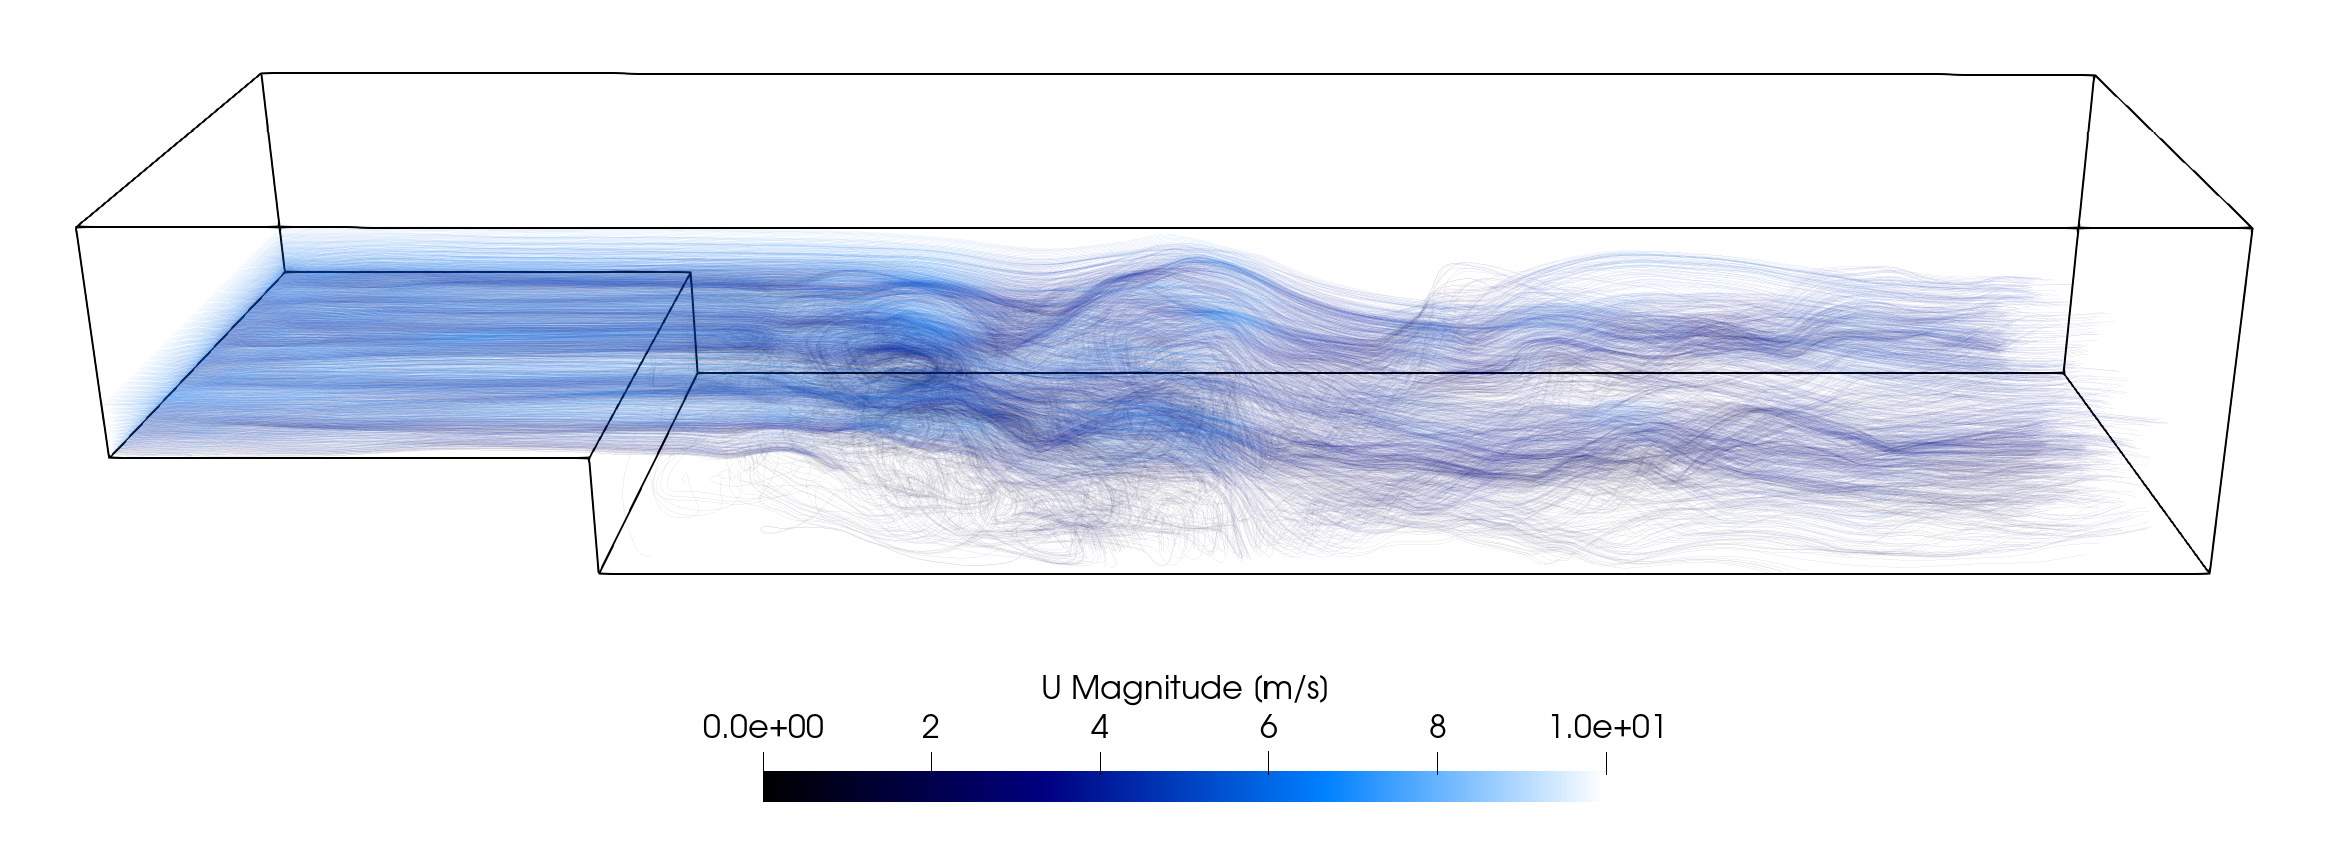
\includegraphics[width=\linewidth]{figures/ch4/BFS_streamlines6.png}
  \caption{Streamlines traced from the entrance of the BFS.}
  \label{fig:BFS_streamlines}
  \end{subfigure}
  \caption{Temperature isocontour of the cross-section(a) and instantaneous streamlines (b) obtained using the \texttt{multiRegionReactingFoam} solver.}
  \label{fig:BFS_contours}
\end{figure}

\begin{figure}
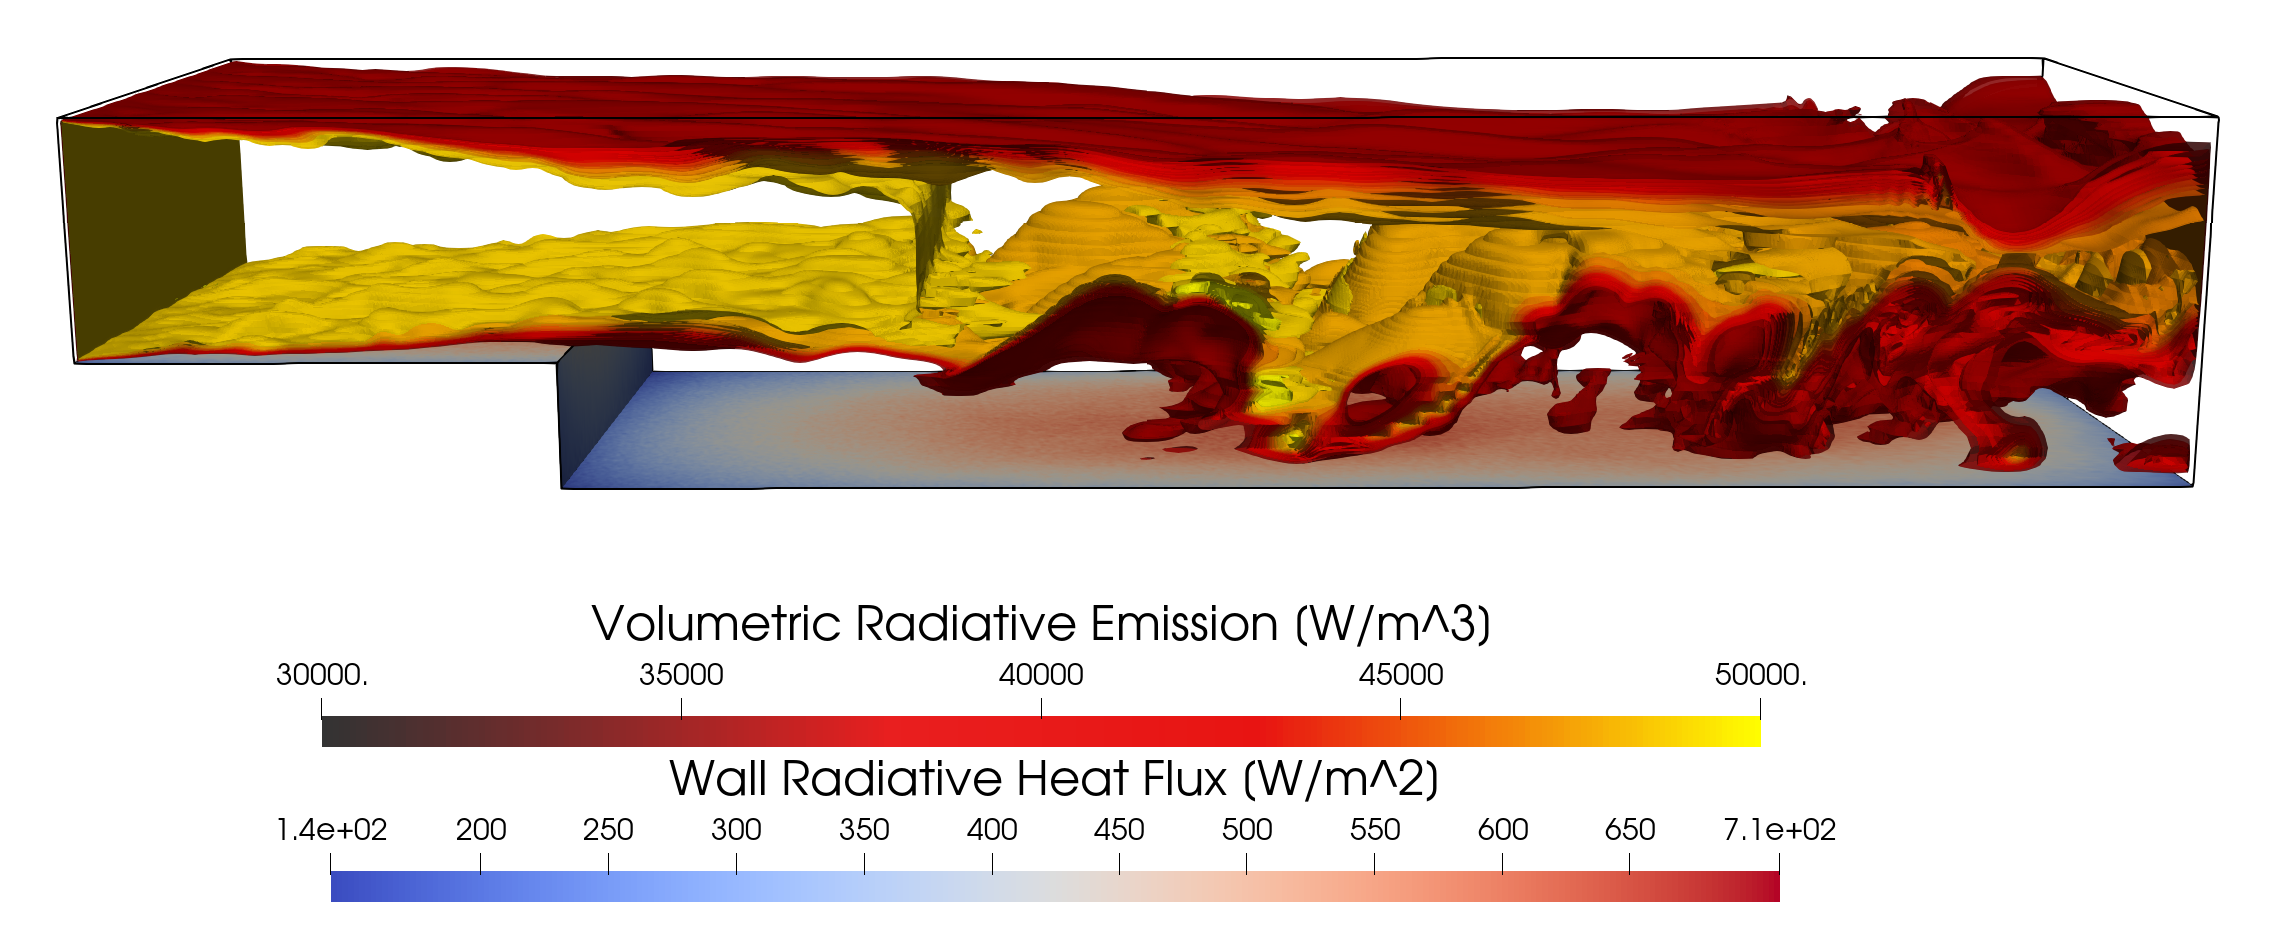
\includegraphics[width=\linewidth]{figures/ch4/BFS_volwallflux3.png}
\caption{Isocontours of volumetric radiative emission alongside resulting radiative heat flux at the walls.}
\label{fig:BFS_radiationcontours}
\end{figure}
The resulting radiative emission and wall-heat flux iso-contours from the MCRT solver are shown in Fig.~\ref{fig:BFS_radiationcontours}.
A small degree of emission is present in the re-circulation zone behind the step. In contrast, the high temperature bulk flow that moves downward halfway aft through the geometry appears to be emitting more significantly.
% The bulk of radiative emission originates from the re-circulation zone behind the step. 
Radiation is emitted from the flow and decreases the thermal energy contained in the passing fluid. 
The fluid is then quickly replaced by the new gas at the entrance, which results in a continuous load of radiation incident on the bottom surface of the domain. 
% The recirculation zone is apparent in the temperature emission contour as a result . The secondary recirculation zone immediately present adjacent to the step displays lower levels of radiative emission resulting from its slower rate of fresh-gas replenishment.

Figures \ref{fig:BFS_RadAbsEmi}, and \ref{fig:BFS_RadSrc} show the radiative absorption, emission, and net energy source along the line shown in Fig.~\ref{fig:BFS_geometry} using the different solvers for comparison. 
The radiative participation peaks towards the center section of the geometry. Peak absorption quantities are extremely low under these conditions due to the low temperatures and absorption coefficient. Results from the Standard-Forward implementation compare well to the well-established Fortran implementation. Oscillations are present in the absorption from both solvers because absorption is determined using a stochastic tracing procedure. Oscillations are not present in the emission profiles because emission is calculated directly using Eq.~\ref{eq:EmissionFromVolume}.
The radiation source (absorption–emission) does not show oscillations because the magnitude of the emission component is significantly higher than the magnitude of the oscillating absorption component.


\begin{figure}
  \begin{subfigure}{1\textwidth}
  \centering
  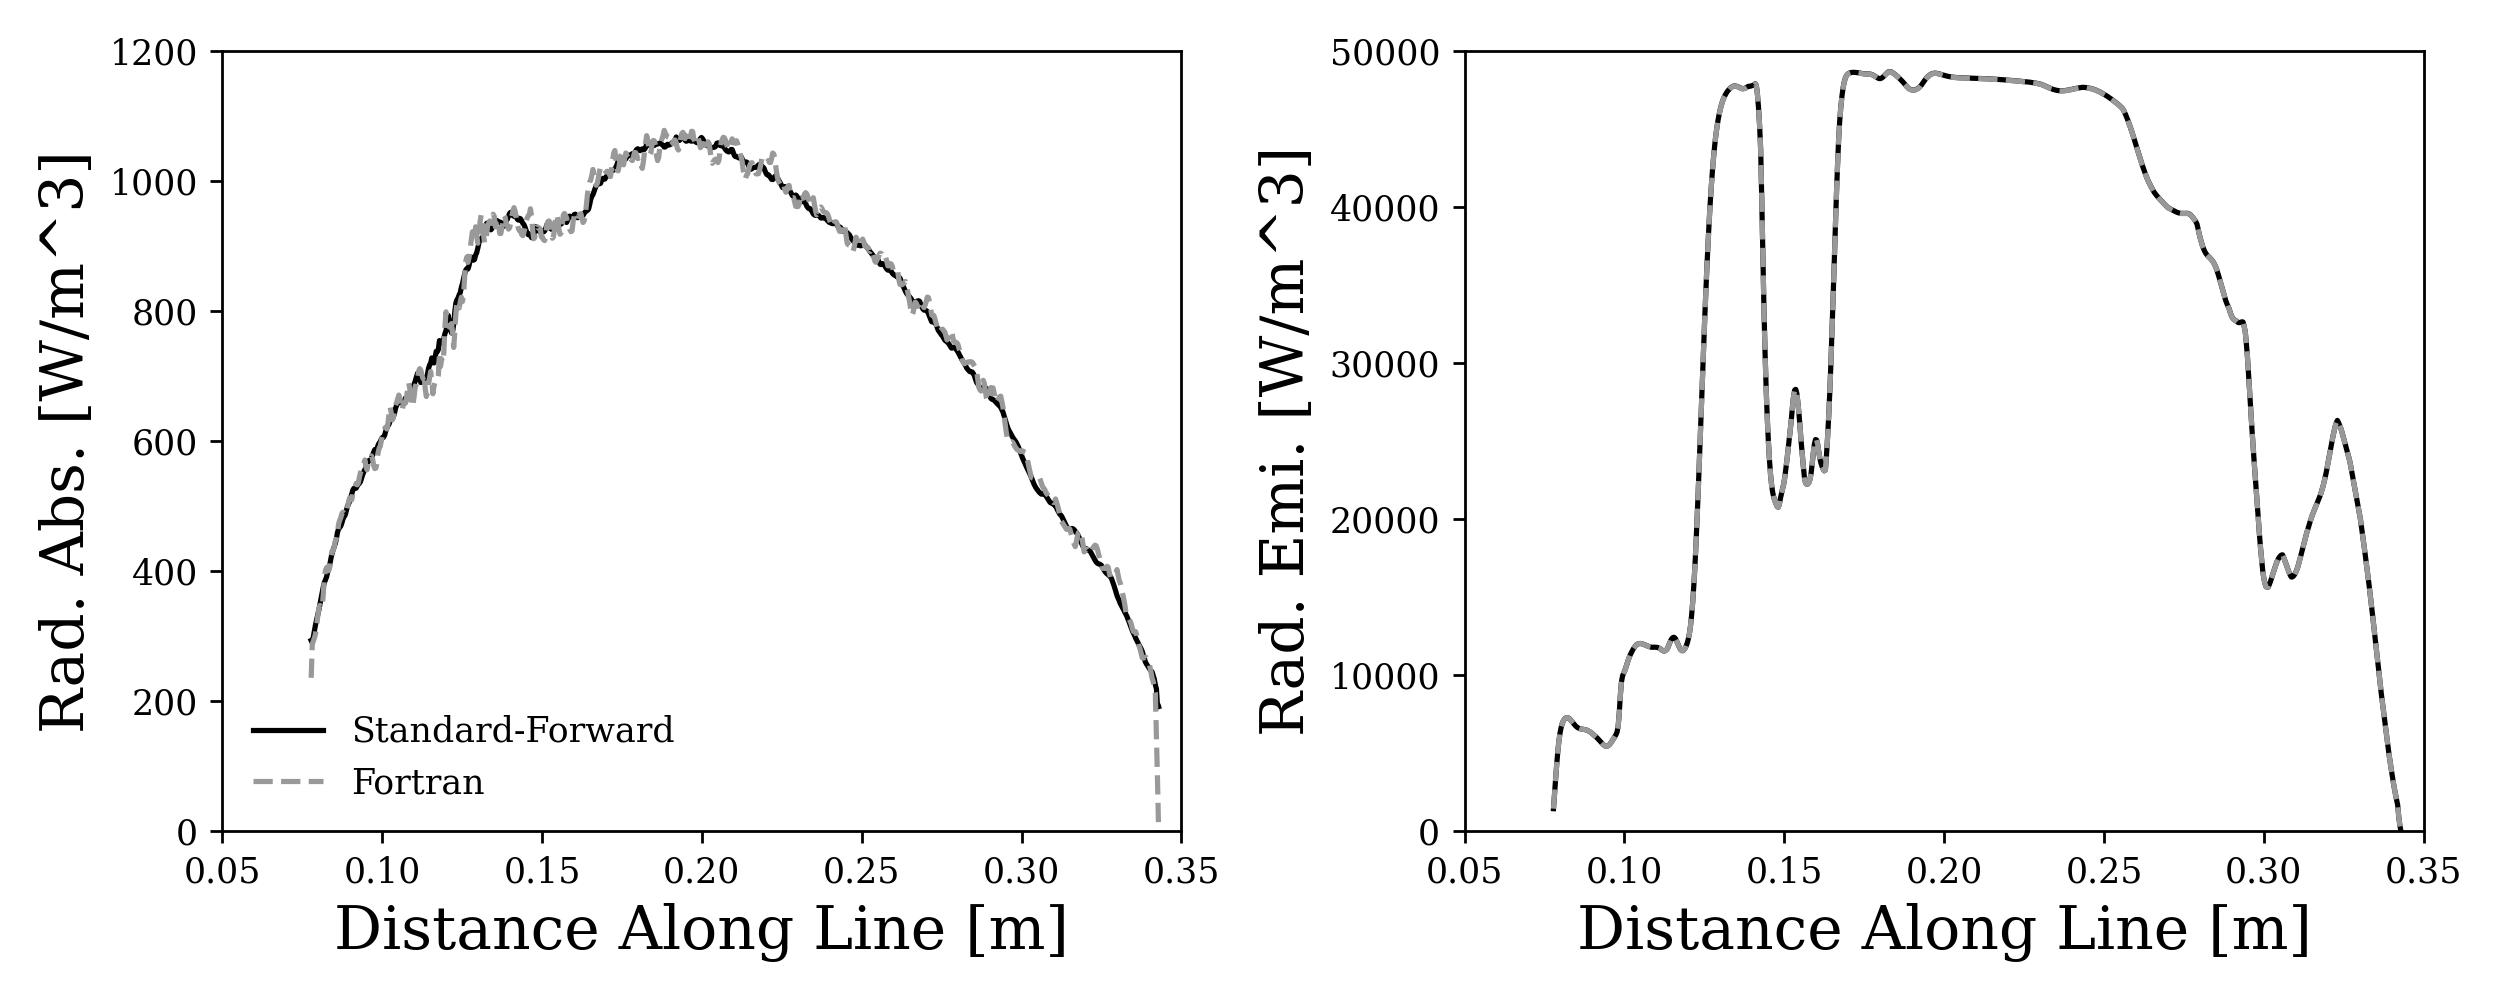
\includegraphics[width=1.0\linewidth]{figures/ch4/BFS_results_top.png}
  \caption{Volumetric radiative absorption and radiative emission sampled along the line present in Fig.~\ref{fig:BFS_geometry}.}
  \label{fig:BFS_RadAbsEmi}
  \end{subfigure}
  % \begin{subfigure}{1\textwidth}
  % \centering
  % 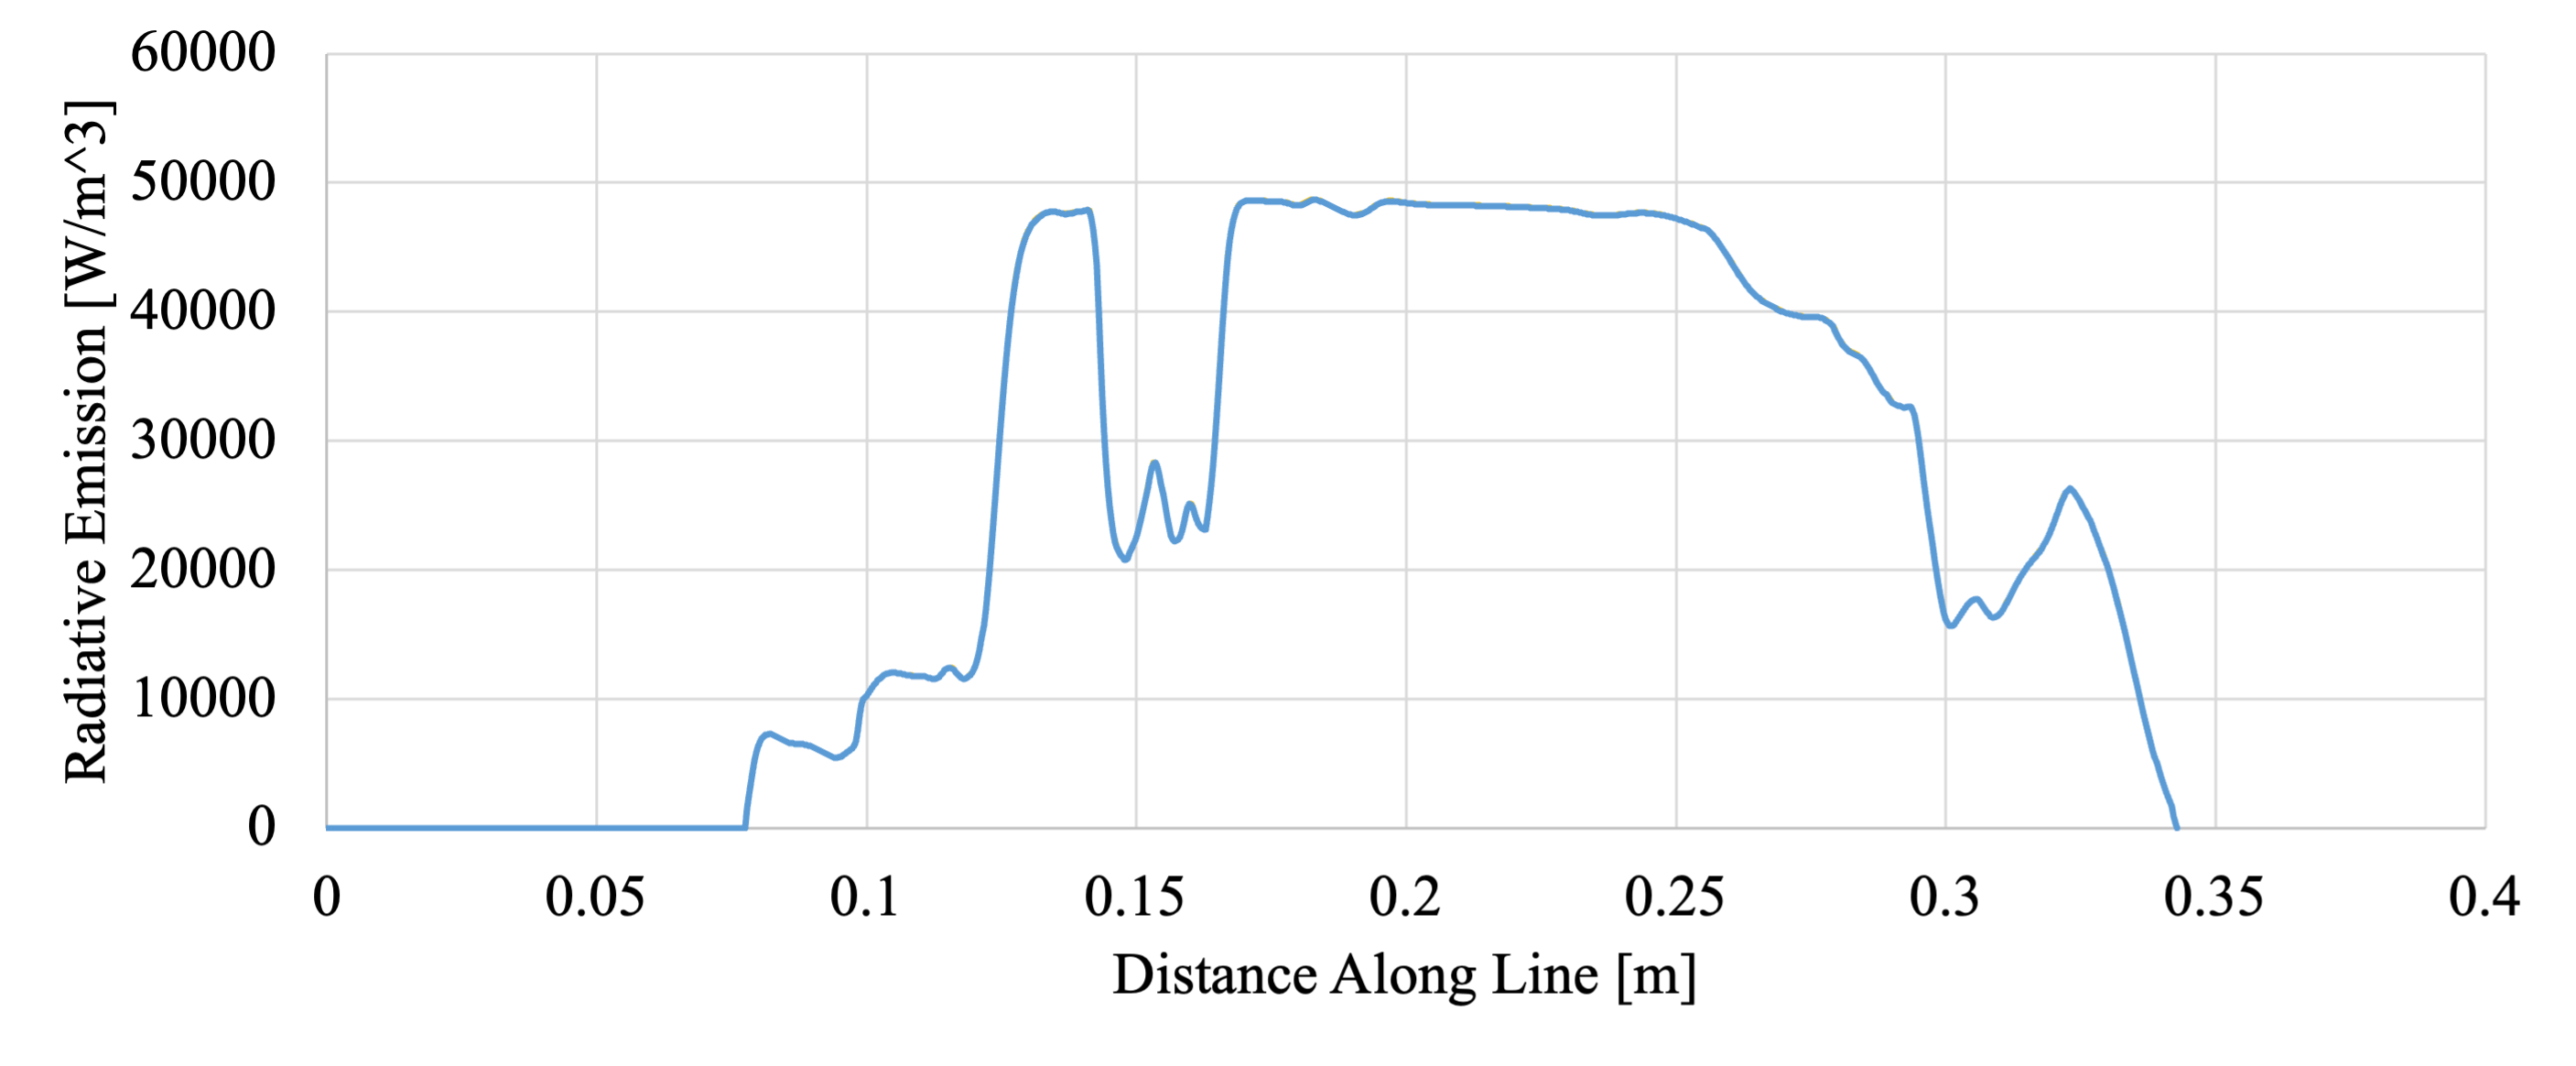
\includegraphics[width=0.8\linewidth]{figures/ch4/LineComparison_RadEmi.png}
  % \caption{Volumetric radiative emission. Same legend as in Fig. \ref{fig:BFS_RadAbs}. All results overlap exactly.}
  % \label{fig:BFS_RadEmi}
  % \end{subfigure}
  \begin{subfigure}{1\textwidth}
  \centering
  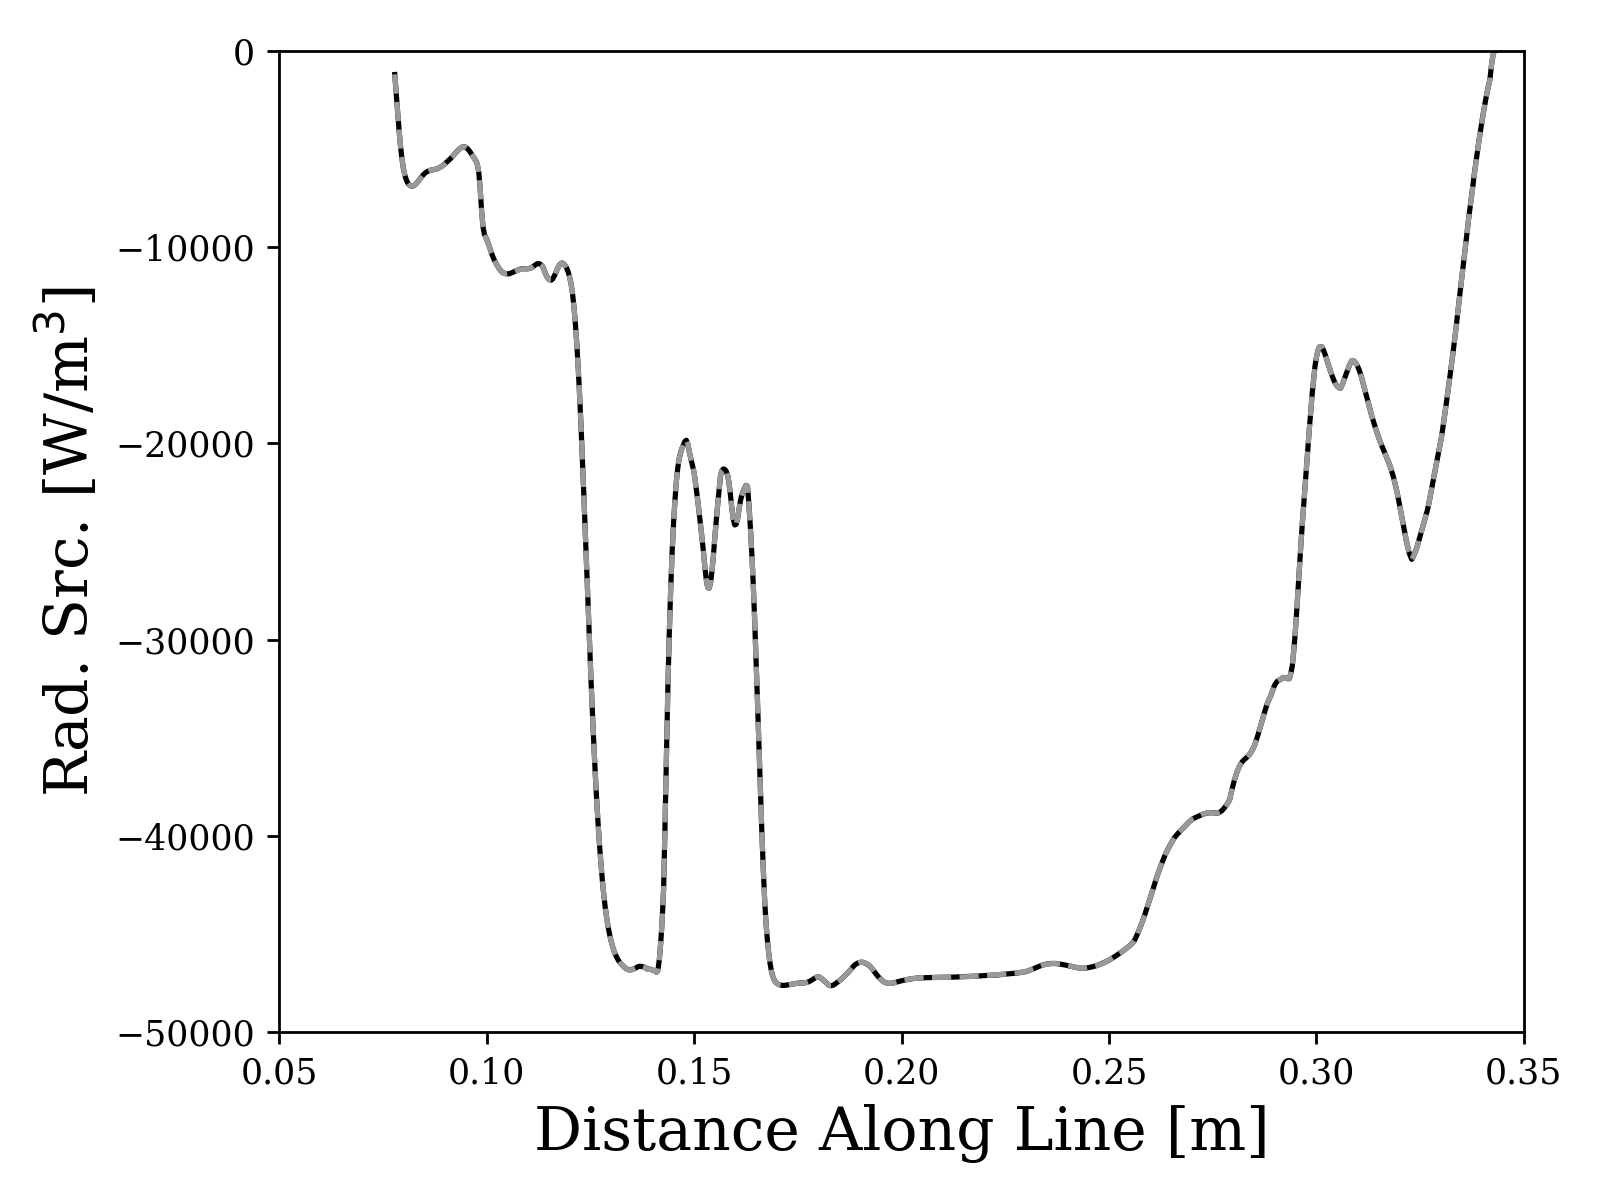
\includegraphics[width=0.55\linewidth]{figures/ch4/BFS_results_bottom.png}
  \caption{Volumetric radiative source term (absorption - emission). Same legend as in Fig. \ref{fig:BFS_RadAbsEmi}.}
  \label{fig:BFS_RadSrc}
  \end{subfigure}
  \caption{MCRT solution results between the present MCRT solver and a well-established Fortran solver of the present backward-facing step after $1.094$ seconds of physical time.}
  \label{fig:BFS_contours}
\end{figure}



\subsection{Model Performance}
Simulation runtimes are presented for the Standard-Forward and Fortran-based solvers. Simulations were performed on the single time-step using 1 ray per cell and 10 rays per cell for all solvers, and serial, OpenMP and Cuda were tested as Kokkos backends for the new MCRT solver. 
% Simulations were performed using a 36-core Intel Xeon Gold 5220 CPU shared-memory workstation for all CPU-parallel computations, and GPU calculations were performed using NVIDIA V100 from the high performance computer Narwhal operated by the U.S. Navy DoD Supercomputing Resource Center with GPU tasks deployed from host AMD EPYC 7H12 CPUs.
Simulations were performed using a single 64-core AMD EPYC 7713 CPU node for all CPU-parallel computations, and GPU calculations were performed using NVIDIA V100 and NVIDIA A100 GPUs from the high performance computer Hornet at the University of Connecticut with GPU tasks deployed from a host AMD EPYC 7452 CPU.


Results are listed in tables \ref{table:BFS_runtime_table_1rpc} and \ref{table:BFS_runtime_table_10rpc} for 1 ray emitted per cell and 10 rays per cell, respectively. The performance of the Standard-Forward model is comparable to the Fortran code model for a serial calculation. A runtime improvement of 31\% is observed before any parallel routines have been applied due to the improved mesh-transfer method implemented in the new MCRT methods. 
Almost no mesh data is duplicated during the mesh transfer process, allowing for minimal delay before the raytracing procedure begins.

\begin{table}
\centering
\caption{BFS runtime comparisons with 1 ray emitted per computational cell.}
\begin{tabular}{c c c c c} 
 \hline
  & Serial & 128 OpenMP threads & V100 GPU & A100 GPU \\ [0.5ex] 
 \hline % 52.3 MPI time
 Fortran & 777.6 s &  N/A & N/A & N/A \\ 
 Standard-Forward & 726.2 s & 38.2 s & 8.0 s & 4.3 s \\
 \hline
\end{tabular}
\label{table:BFS_runtime_table_1rpc}
\end{table}

\begin{table}
\centering
\caption{BFS runtime comparisons with 10 rays emitted per CFD cell.}
\begin{tabular}{c c c c c c} 
 \hline
 & Serial & 128 OpenMP threads & V100 GPU & A100 GPU \\ [0.5ex] 
 \hline
 Fortran & 7421.7 s & N/A & N/A & N/A \\%& 301.0 \\
 Standard-Forward & 6867.8 s & 402.7 s & 55.4 s & 23.7 s \\%& 82.5 \\
 \hline
\end{tabular}
\label{table:BFS_runtime_table_10rpc}
\end{table}



The introduction of a parallel back-end results in dramatic speedups. With 128 OpenMP processes, the Standard-Forward method reduces runtime by 19 times over serial and 20 times over the Fortran-based code with one ray emitted per computational cell.
% The Fortran code exhibits a large speedup due to its parallel ray-tracing procedure. Also, because OpenFOAM will load different sections of the mesh on different processors simultaneously when MPI parallelism is used, the mesh initialization process in the Fortran code is significantly reduced. An identical reduction would be found for Standard-Forward when run with MPI.
% Within Standard-Forward, runtimes are decreased. This can be attributed to the longer mesh initialization time resulting from the usage of a single MPI process.
The usage of a GPU enabled an even greater reduction in runtime. Speedups of 169 and 290 are observed when using the A100 GPUs for the 1 ray per cell case and 10 rays per cell case, respectively.

\section{Direct Numerical Simulation of a Turbulent Pool Fire}\label{section:DNSPoolFire}
% Turbulent pool fire
With successful validation of the solver under 1-D and 3-D configurations, the solver is then tested on a non-gray direct numerical simulation of a turbulent pool flame. The pool flame is a canonical configuration used in the field of fire research as a surrogate for many hazardous combustion scenarios~\cite{Chen2023PoolAdvances}. 
The flame is a non-premixed turbulent diffusion flame where fuel is supplied through the inlet on the bottom face and buoyant forces drive the high-temperature, reacting flame to rise up and puff periodically.
Furthermore, the high temperatures from the chemical reaction alongside the larger length scales provide high radiative emissions with higher optical thickness compared to laboratory jet flames such as the Sandia D flame~\cite{Barlow1998EffectsFlames}. For the present study, the configuration is tested first using the Monte Carlo code using a line-by-line non-gray model with various hardware back-ends. 
Next, a gray model is used in the MCRT solver to allow for a fair comparison against existing finite volume Discrete Ordinates Method (fvDOM) and P-1 models embedded in \texttt{OpenFOAM}.

\subsection{Case Setup}
The simulation geometry, mesh, and case conditions are identical to those of Ref.~\cite{Wu2020DetailedFire} where the Fortran based Monte Carlo ray tracing solver was applied with a line-by-line non-gray model~\cite{Ren2019Line-by-lineSystem} for a DNS. The original simulation was conducted using an in-house \texttt{reactingDJFoam} solver within \texttt{OpenFOAM}~\cite{Wu2019AFlame} and consisted of an n-heptane/air non-premixed turbulent flame. The geometry is presented in Fig.~\ref{fig:PoolFireVisual}. The mesh resolution is $9.6$ million hexahedral cells in a cylindrical domain of diameter $0.781$ m and height $0.600$ m. The pool is centered and has a diameter of $7.1$ cm. The grid resolution is approximately $1$ mm in the axial direction and $0.5$ mm in the radial direction with additional refinement around the pool location. The Kolmogrov scale is approximately $0.5$ mm, which is considered resolved in this study, and subgrid modeling is not included in the original simulation. 
%Turbulence-radiation interaction (TRI) and sub-grid modeling are not included in neither the original simulation nor the present frozen-field analysis. 
The flame itself is a highly sooting flame with a radiant fraction of 29\%~\cite{Wu2020DetailedFire}. 


\begin{figure}[!b]
\centering
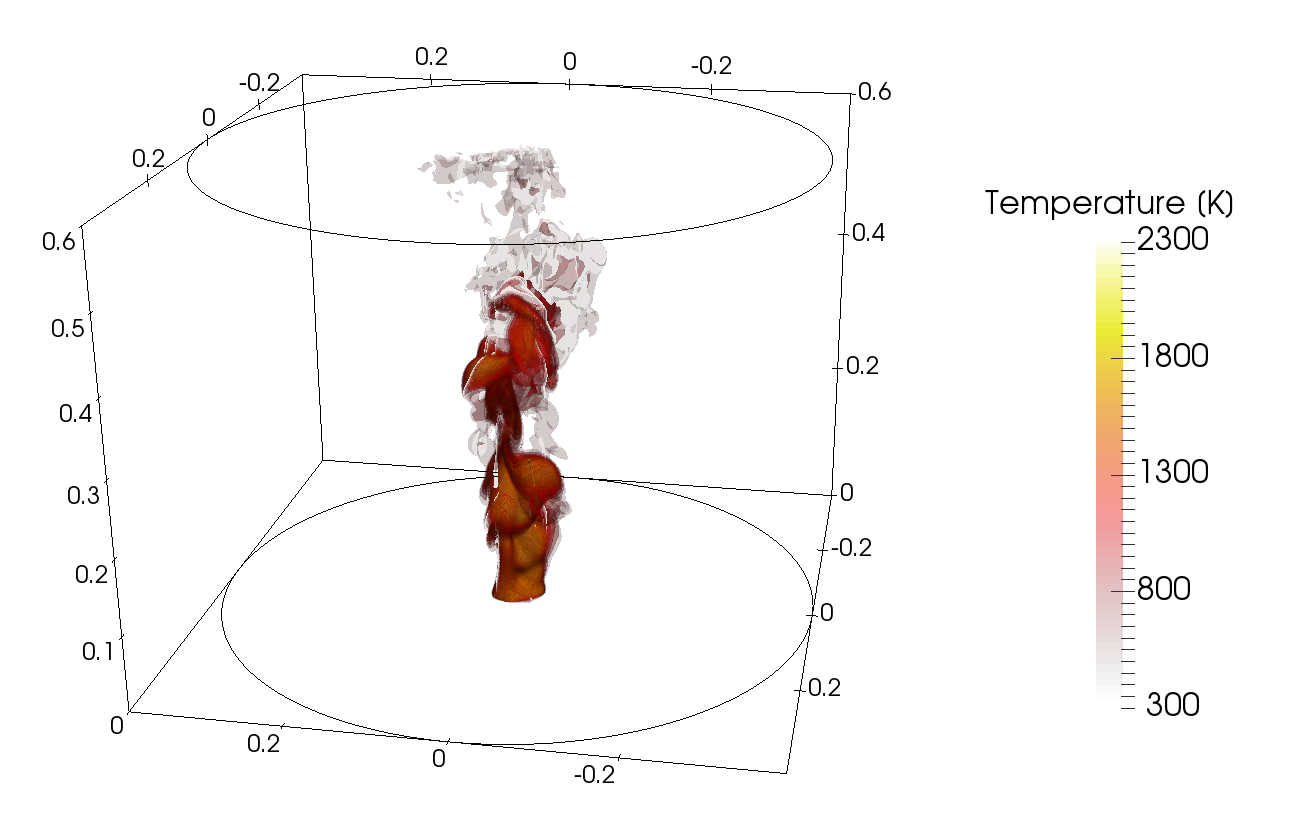
\includegraphics[width=0.8\linewidth]{figures/ch4/PoolFireVisual.png}
\caption{Instantaneous temperature isocontour from the turbulent pool fire used for runtime analysis in this study. The dimension of the geometry is also illustrated.}
\label{fig:PoolFireVisual}
\end{figure}


\begin{figure}[!b]
\centering

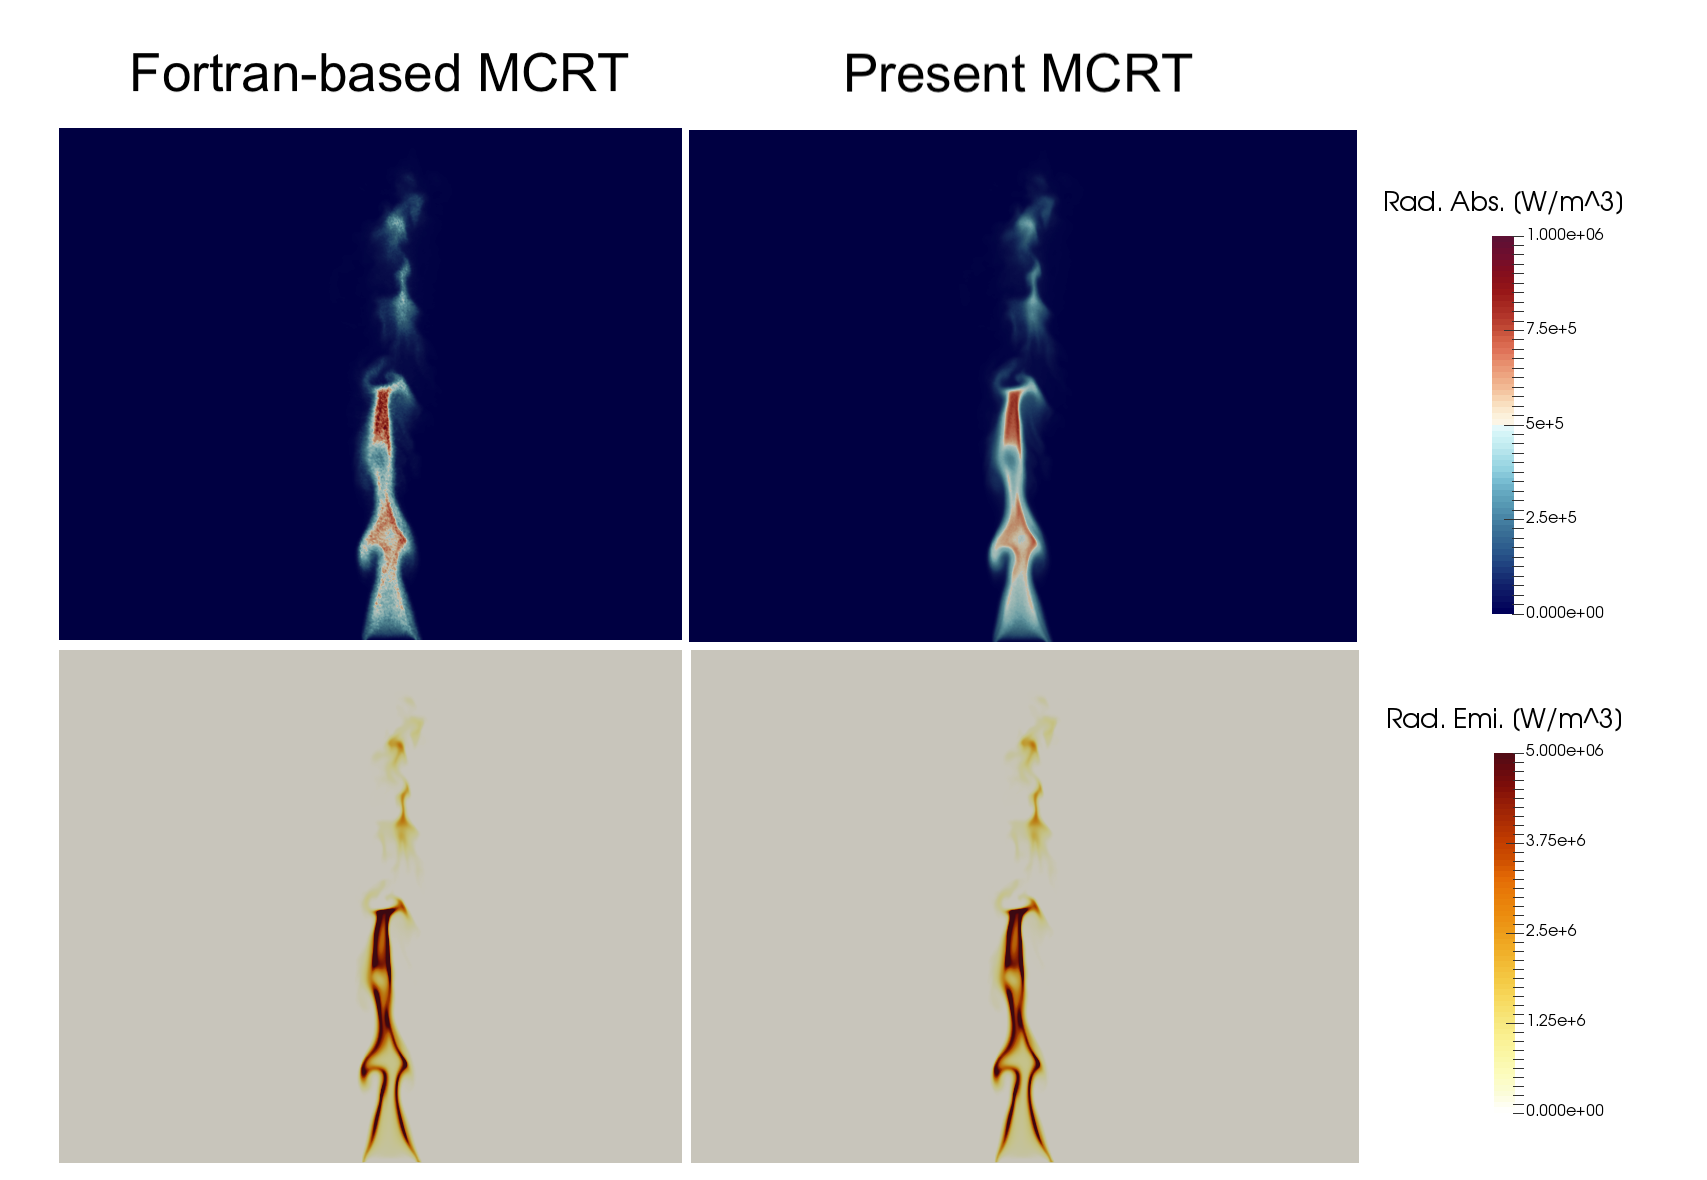
\includegraphics[width=0.7\linewidth]{figures/ch4/PoolFire_Verification.png}
\caption{Mid-plane contours of radiative emissive power and radiative absorption from the Fortran-based solver used in Ref.~\cite{Wu2020DetailedFire} and the present solver.}
\label{fig:PoolFireVerificationColor}
\end{figure}


\begin{figure}[!bh]
\centering

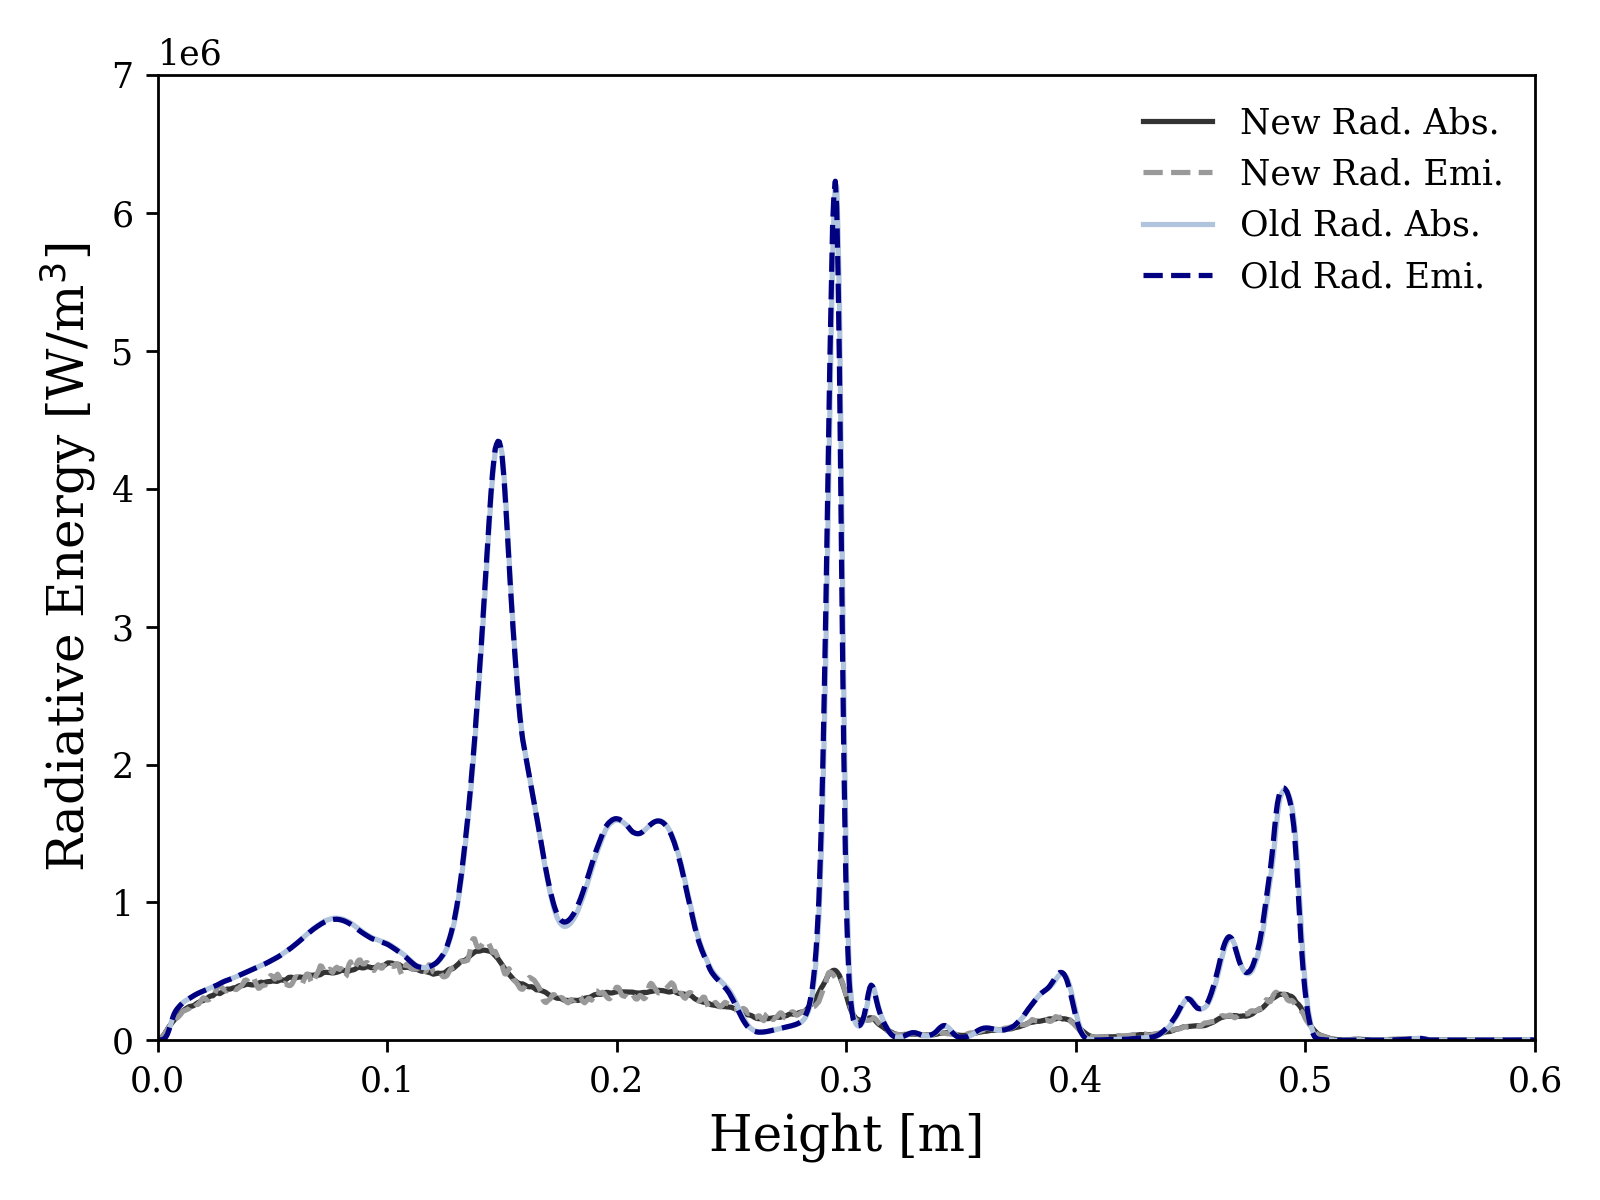
\includegraphics[width=0.7\linewidth]{figures/ch4/lineplot_verification.png}
\caption{Centerline radiation source term with line-by-line non-gray radiation from the present MCRT solver and the Fortran-based MCRT solver.}
\label{fig:PoolFireVerificationLine}
\end{figure}

The present study solves radiation for a single snapshot at exactly $1.25$ s of physical time. Time is frozen, and the ray-tracing procedure is conducted within a static field. The adaptive radiative emission model is used where the number of rays emitted from a cell scales proportionally with the cell's radiative emissive power~\cite{Wang2007AnFields}, as per section~\ref{section:adaptiveemission}. This resulted in a total of $103,907,333$ rays emitted, with most emission occuring from within the flame. Twenty solutions to the radiation transport equation are evaluated using MCRT and averaged over to obtain mean solver runtimes.
%, with the exception of the serial run where five solutions are used. 
Non-gray CO$_2$, H$_2$O, CO, and soot are modeled using a line-by-line model of Ref.~\cite{Ren2019Line-by-lineSystem}. 

\subsection{Verification and Performance of line-by-line MCRT}
To verify the new radiation solver with the line-by-line database,
Fig.~\ref{fig:PoolFireVerificationColor} visually compares the radiative emissive power and radiative absorption across the centerplane between the new MCRT solver and the previous one used in Ref.~\cite{Wu2020DetailedFire}. One ray per cell was emitted for each computational cell in Ref.~\cite{Wu2020DetailedFire} and radiation was solved on the fly in that study. Identical line-by-line tables are employed in both studies. 
% Good agreement is observed between the two solvers.
Figure~\ref{fig:PoolFireVerificationLine} further presents a more quantitative comparison along the centerline of the pool. The agreement in both the emission and absorption source terms is excellent, with more fluctuations in the absorption source observed from previous results because fewer rays were used in that study. 

Radiation execution times are presented in Table~\ref{table:PoolFireRuntimes} for various \texttt{Kokkos} back-ends. No changes to the radiation code are made across the various hardwares tested. Both CPU and GPU parallelism display a significant speedup over serial CPU calculations.
The NVIDIA A100 GPU requires approximately $1/400^{\text{th}}$ of the computational time to simulate an equivalent radiation problem as one CPU thread running in serial. Likewise, the V100 also shows speedups greater than two orders of magnitude. Interestingly, the NVIDIA A100, released in 2020, shows a greater than two times speedup over the NVIDIA V100, released in 2017. Meanwhile, OpenMP with the AMD Epyc 7713 CPU shows speedups an order of magnitude faster than serial and an order of magnitude slower than the A100 GPU.

Run-times are also presented with MPI enabled on 2 ranks, both MPI ranks are present in the aft direction. The two MPI ranks are situated on separate computing nodes with different NVIDIA A100 GPUs. Run-time decreases because of the greater resources present. The decrease is limited, however, because of the additional MPI communication overhead incurred. Future work will integrate the Hybrid-Reverse algorithm in this configuration to improve multi-rank scalability.

\begin{table}
\caption{Comparison of MCRT runtimes with line-by-line radiation for a single snapshot of a DNS of a turbulent pool-fire.}
\label{table:PoolFireRuntimes}
\centering
\begin{tabular}{c c c c c c c} 
 \hline
 ~ & A100 GPU & V100 GPU & OpenMP & Serial & A100/2ranks \\ [0.5ex] 
 \hline
 % A100 $($\pm{}$5.3), V100 ($\pm$57.0), OMP pm 225
 Runtime & 117.9 s & 278.0 s & 1333.3 s & 44844.5 s & 102.2 s \\ 
 Speedup over serial & 380 & 161 & 34 & 1 & 439 \\
 Speedup over OpenMP & 11 & 5 & 1 & 0.03 & 13 \\
 \hline
\end{tabular}
\end{table}

% Under identical conditions the solver is then run with multiple MPI ranks. The domain is split into a total of 32 MPI ranks, 8 in the aft direction and 4 axi-symmetric axis-aligned quadrants.  are  The Standard-Forward and Hybrid-Reverse methods are tested and their runtimes are compared.


\subsection{Comparison with other radiation solvers using a gray model}


The pool-fire simulation is then employed to compare the new MCRT solver with other popular solvers including the fvDOM solver and P-1 solver from \texttt{OpenFOAM-5.x}. A constant absorption coefficient of $0.5$ 1/m is prescribed to each computational cell in the same snapshot to maintain identical spectral models between all solvers. 
Adaptive emission is turned on for the MCRT method resulting in 101,000,825 total rays. The fvDOM solutions were obtained using \texttt{OpenFOAM} default settings, but with 16 azimuthal discretizations and 4 polar discretizations. 
Each fvDOM solution required 50 iterations to converge to final residuals of $O(10^{-5})$, and $20$ fvDOM solutions were obtained for runtime averaging. Twenty P-1 solutions were also obtained for runtime averaging using OpenFOAM default settings.

A comparison of solutions within the gray medium are presented in Fig.~\ref{fig:PoolFireVerificationLine2}. MCRT and fvDOM show comparable profiles. The P-1 solution shows significant deviation of radiative absorption in both magnitude and shape from the more-accurate MCRT and fvDOM solutions. 
\begin{figure}[!h]
\centering
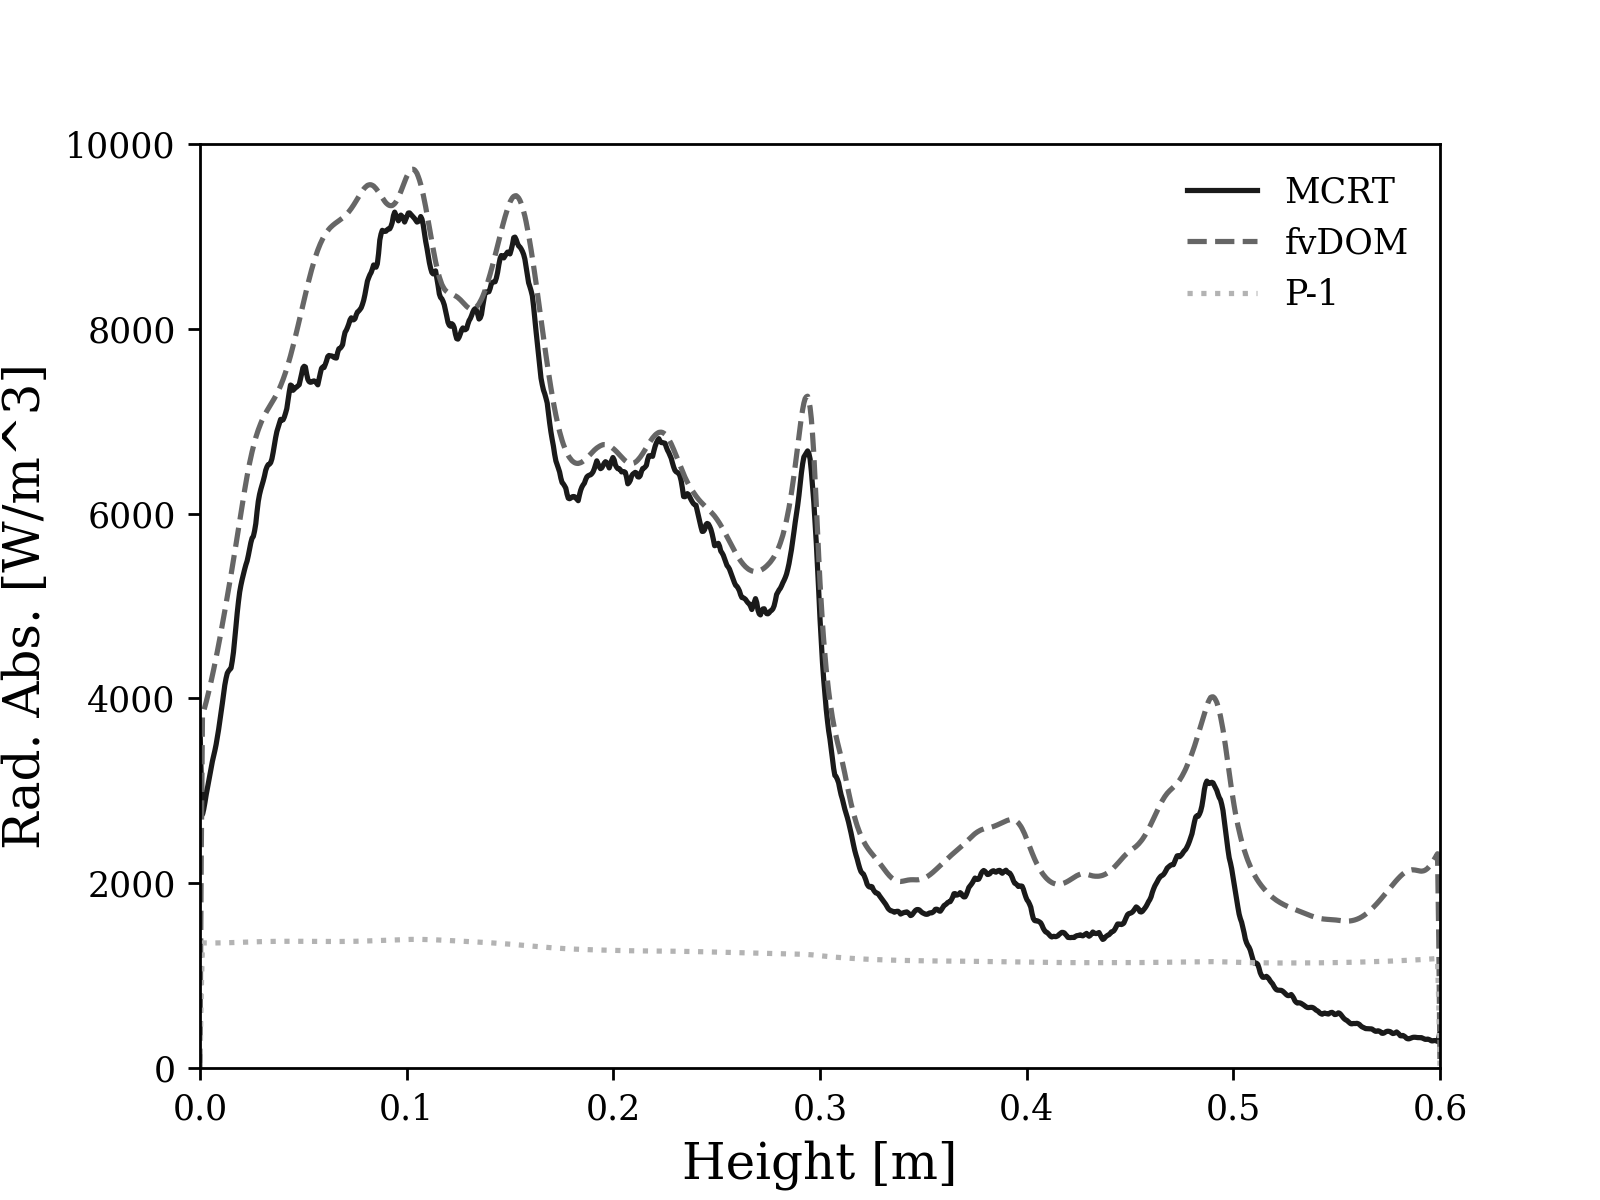
\includegraphics[width=0.6\linewidth]{figures/ch4/comparison_verification.png}
\caption{Centerline radiative absorption with gray radiation from the present MCRT solver and the \texttt{OpenFOAM} fvDOM and P-1 radiation solvers.}
\label{fig:PoolFireVerificationLine2}
\end{figure}

Solver runtimes are presented in Table~\ref{table:PoolFireRuntimesGray}. The GPU accelerated MCRT solver is again shown to improve solver performance significantly over both the serial and OpenMP versions. Moreover, the GPU solution is shown to be faster than fvDOM and, interestingly, the P-1 serial calculations. This indicates that such a GPU-accelerated MCRT solver has great potential to replace some reduced-order solvers and be applied on the fly in combustion simulations.



\begin{table}
\caption{Comparison of MCRT runtimes of gray radiation within a single-snapshot of a DNS of a turbulent pool-fire.}
\label{table:PoolFireRuntimesGray}
\centering
\begin{tabular}{c c c c c c} 
\hline
&\multicolumn{3}{c}{\bfseries MCRT}&\multicolumn{2}{c}{\bfseries OpenFOAM} \\
 \hline
 ~ & A100 GPU & OpenMP & Serial & fvDOM serial & P-1 serial \\ [0.5ex] 
 \hline
 % A100 ($\pm$0.43), omp 224, fvDOM ($\pm{}$708), P1 ($\pm{}$2.4)
 Runtime (s) & 74.3 s & 1070.4 s & 33262.5 s & 4426.3 s & 112.5 s \\ 
 Speedup over fvDOM & 60 & 4 & 0.13 & 1 & 39 \\
 Speedup over P-1 & 1.5 & 0.1 & 0.003 & 0.03 & 1 \\
 \hline
\end{tabular}
\end{table}



\section{Transient Small Pool Fire}\label{section:SmallPoolFlame}
Finally, the solver is applied to a transient turbulent pool-fire, to demonstrate its feasibility of coupling with CFD applications. Similar to the study of section~\ref{section:DNSPoolFire}, the domain consists of turbulent non-premixed flame fueled by a circular fuel source along the bottom face. However, unlike the previous study, radiation is fully coupled to fluid dynamics from its initial conditions, and radiation quantities are directly extracted from the simulation. 

\subsection{Case Setup}
The simulation is based on a \verb|OpenFOAM-5.x| tutorial case, \texttt{smallPoolFlame3D}, where mesh refinement has been doubled and the default discrete-ordinates radiation model has been deactivated. 
In the tutorial case, a mass-source is provided through the inlet at the bottom of the domain, where a reaction is also initiated. A turbulent non-premixed flame is then simulated with infinitely-fast chemistry for four seconds of physical time.
Both a frozen-field analysis on a single-timestep and a full transient simulation are conducted and analysed. The single-timestep analysis is conducted using the original \texttt{smallPoolFlame3D} \verb|fireFoam| tutorial case, but with radiation turned off, and the timestep is obtained at 0.8s of physical time and is shown in Fig.~\ref{fig:PoolFire_diagram}.

The geometry is a cubic 1$\times$1$\times$1m domain with a grid consisting of 1,728,000 hexahedral cells with 120 divisions per side.
The size of the pool fire is much larger than the pool fire presented in section 4.3 and is not feasible to be modeled by DNS.
This configuration is studied for both planck-mean gray and line-by-line spectral models, and no turbulence-radiation interaction (TRI) is accounted for in this study. %IS THIS A DNS?

\begin{figure}
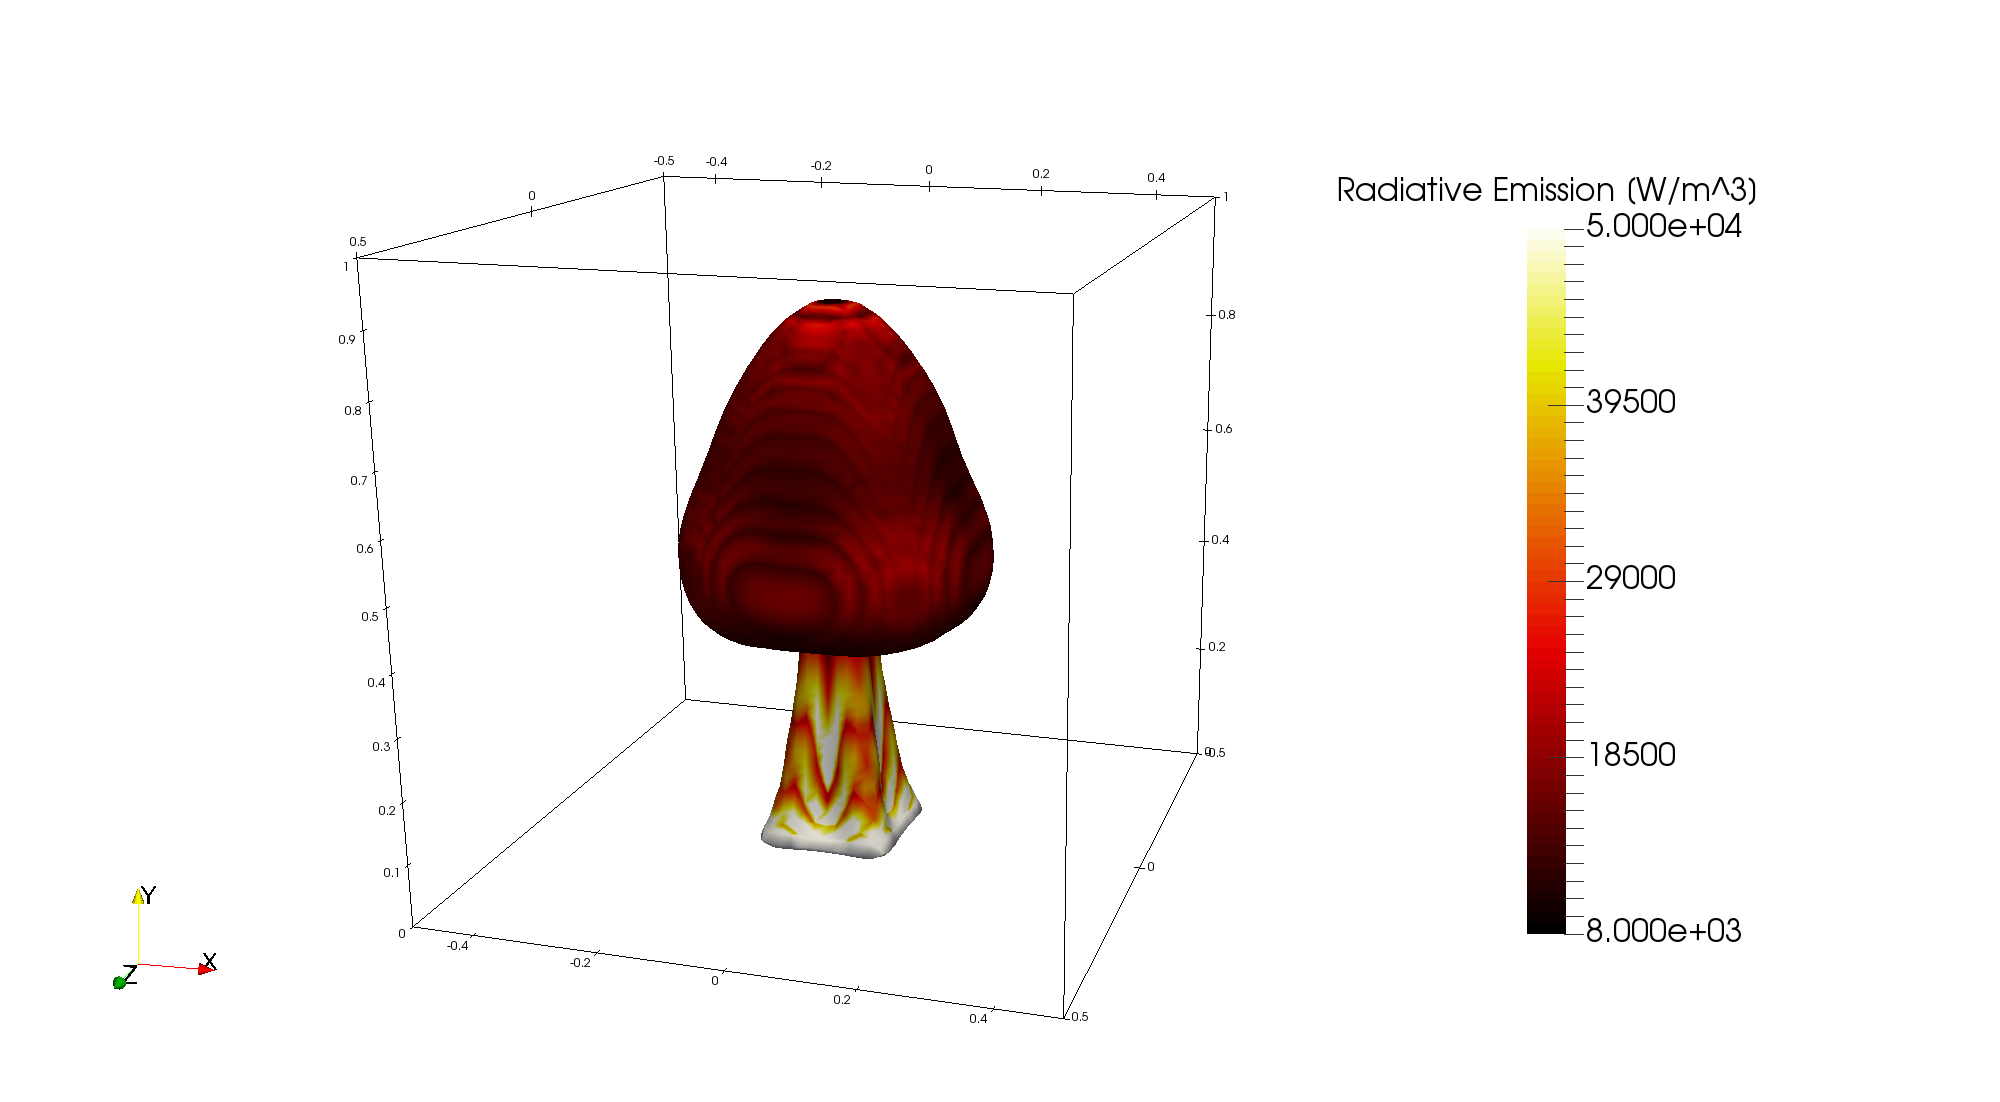
\includegraphics[width=\linewidth]{figures/ch4/contour_early.png}
\caption{An early timestep of the pool fire flame simulation. Isosurface is 0.03 CO$_2$ mass fraction colored by velocity magnitude in meters per second. Axes dimensions are in meters.}
\label{fig:PoolFire_diagram}
\end{figure}

\subsection{Results}
Figure \ref{fig:PoolFire_radiationcontours} displays the radiative emission and wall absorption patterns for the flame. Wall heat flux is maximized near the inlet section, directly adjacent to the location of ignition. 
The radiative emission contours drop towards the outer edges and top section of the mushroom-like shape. The turbulent mixing of the reacting flow with surrounding quiescent fluid results in a reduction in temperature and decreased volumetric emission.  

\begin{figure}
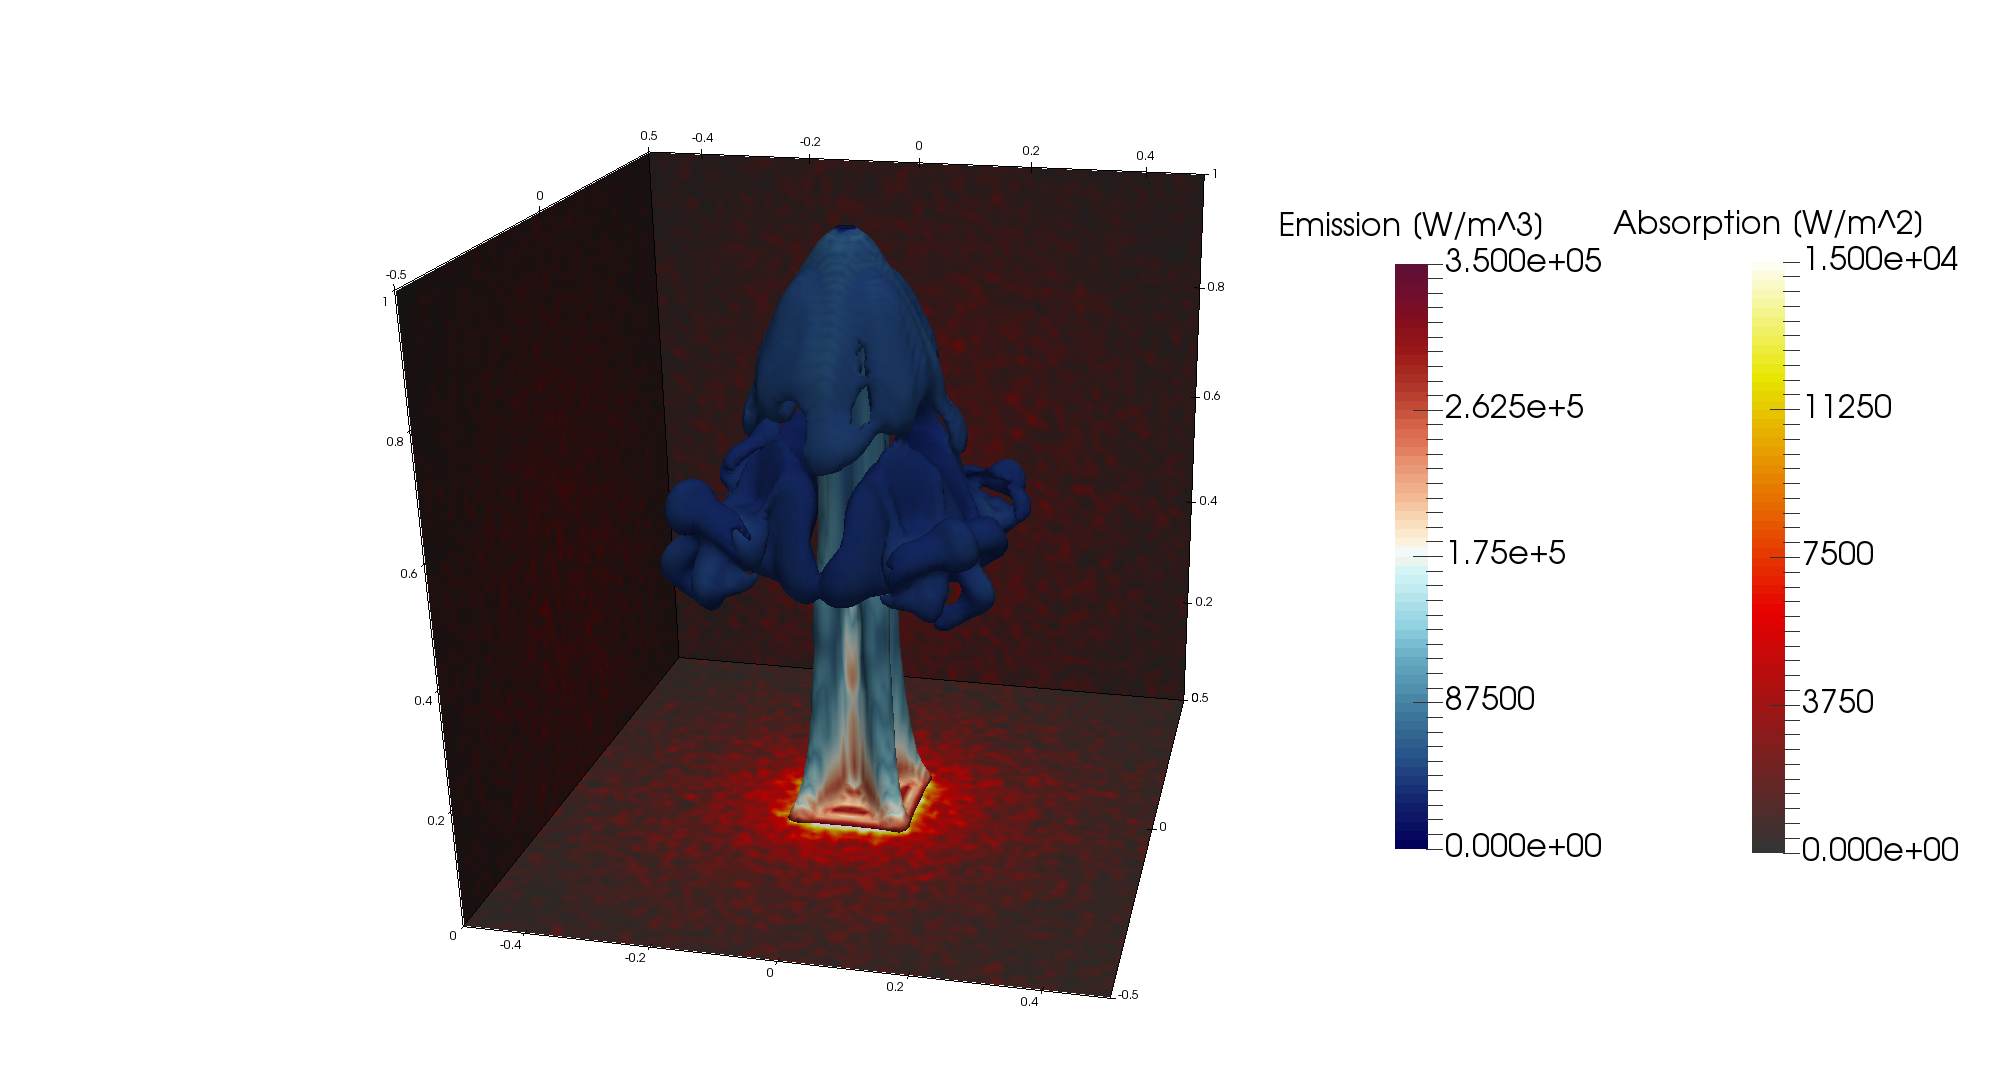
\includegraphics[width=\linewidth]{figures/ch4/radiation_contours.png}
\caption{Isosurface of 0.03 CO$_2$ mass fraction colored by radiative emission. Wall coloring represents wall radiative heat flux.}
\label{fig:PoolFire_radiationcontours}
\end{figure}

% \subsubsection{Single Timestep}
% A single timestep from the original smallPoolFire3D simulation is extracted and radiation is simulated.
% In order to better understand the influence of radiation within the flame, Fig. \ref{fig:PoolFire_quadcomparison} displays four radiation relevant parameters for the MCRT calculation within the frozen field analysis. 
% The contours of temperature show two sides of a hollow cylinder of reacting flow billowing upwards as a result of the buoyant force induce on the lower-density regions.
% The top-section of the mushroom contains a flame-front which, towards the outer regions, slowly decreases in temperature and intensity as a result of momentum and molecular exchange with the surrounding quiescent region through viscous and diffusive effects.
% High temperature regions correlate strongly with the points of high emission, and the wings of the mushroom show a much stronger decay in emission as a result of the fourth power dependence of radiative emission with temperature.

% \begin{figure}
% \centering
% 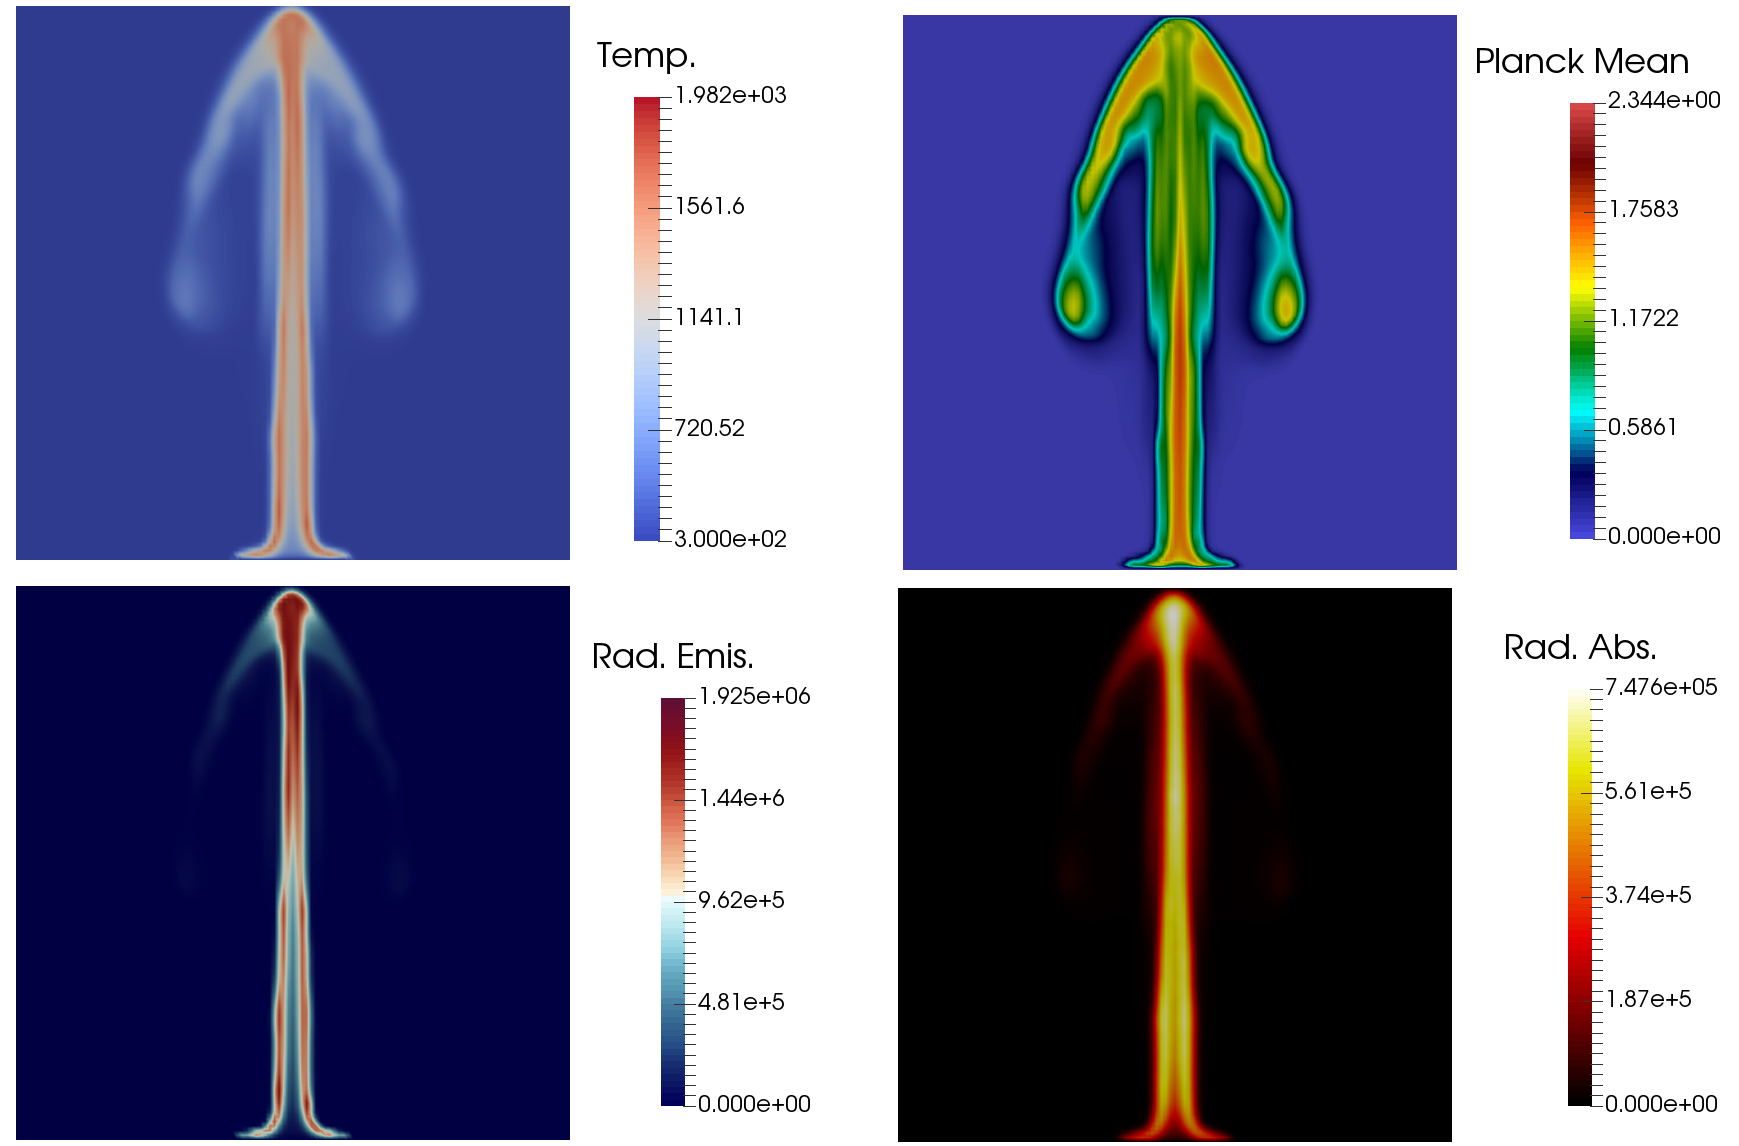
\includegraphics[width=0.85\linewidth]{figures/ch4/PoolFire_quadcomparison.png}
% \caption{Mid-plane contours of four relevant parameters to the radiation calculation in the pool fire. Temperature is in Kelvin, Planck Mean absorption coefficient is in m$^{-1}$, and radiative emission and absorption are in W/m$^3$.}
% \label{fig:PoolFire_quadcomparison}
% \end{figure}

% Absorption visually appears to correlate much more closely with the Planck-mean absorption coefficient than temperature. Absorption is maximized near the entrance region of the flame, and maintains its strength throughout the tight upwards-moving stream of fluid.
% The significant drop in Planck-mean absorption coefficient with radiative absorption in the non-reacting regions of the flow suggests that the flame is responsible for the bulk of radiative re-absorption. 

% In total, net radiative emission equals $10541.5044$ Watts, where $1469.4406$ Watts are re-absorbed into the medium, and $9072.0639$ Watts escape to the walls. This results in approximately 14\% of radiative emission being re-absorbed, primarily in the flame-region, as suggested previously. 
% The maximum volumetric radiative energy loss for any computational cell is -$1.081$ W. In comparison, the maximum volumetric source through chemical reaction was $14.08$ Watts.

% Figure \ref{fig:PoolFire_lineplot} shows various normalized parameters along the center-line of a gray-simulated flame. 
% Normalized temperature and product species mass fractions rise with increasing distance from the bottom surface, indicating reaction progression. 
% The volumetric emission and negative of radiative volume source (emission – absorption) appear to match as a result of the relatively weak influence of absorption.
% The Planck Mean absorption coefficient increases, then decreases despite the monotonically increasing mass fractions of the radiatively participating species (CO$_2$ and H$_2$O). This happens as a direct result of the increase in temperature. 
% The influence of temperature on absorption coefficient is complex, but for these conditions the rotation partition function of molecular energy states of the participating species is responsible for the decrease of absorption coefficient at this temperature range~\cite{Modest2013RadiativeTransfer}.
% Absorption follows the trend of planck-mean absorption coefficient, as expected for an gray model.

% Figure \ref{fig:PoolFire_lineplot_nongray} displays the same normalized parameters in a LBL-accurate Pool-fire simulation. The contributions of CO$_2$ and H$_2$O are considered, but not soot.
% The most notable changes are the inversion of the radiative absorption profile. Absorption now increases with height in the flame. Line-by-line accuracy means that the rate of absorption is decided by the wavelength of the ray.
% This results in an increase of re-absorption as the rays with wavelengths of high rates of absorption are also preferentially selected during the random wavenumber selection process. This results in a net increase of radiative re-absorption from $14$\% for the gray flame to $58$\% for the non-gray flame.
% The resulting negative radiation source contour shown in Fig.~\ref{fig:PoolFire_lineplot_nongray} also reflects this change by showing a slight degree of absorption towards the lower-sections of the flame.

% \begin{figure}[!ht]
% 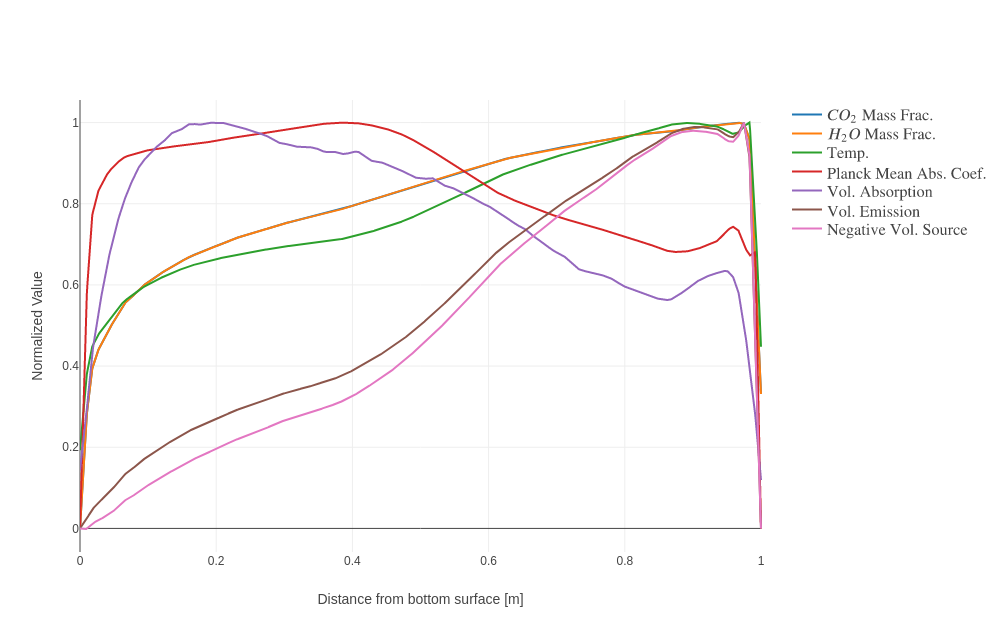
\includegraphics[width=\linewidth]{figures/ch4/line_plot.png}
% \caption{Various parameters along the center-line of a gray flame. Values normalized by maximum values along the sampled line.}
% \label{fig:PoolFire_lineplot}
% \end{figure}


% \begin{figure}[!ht]
% 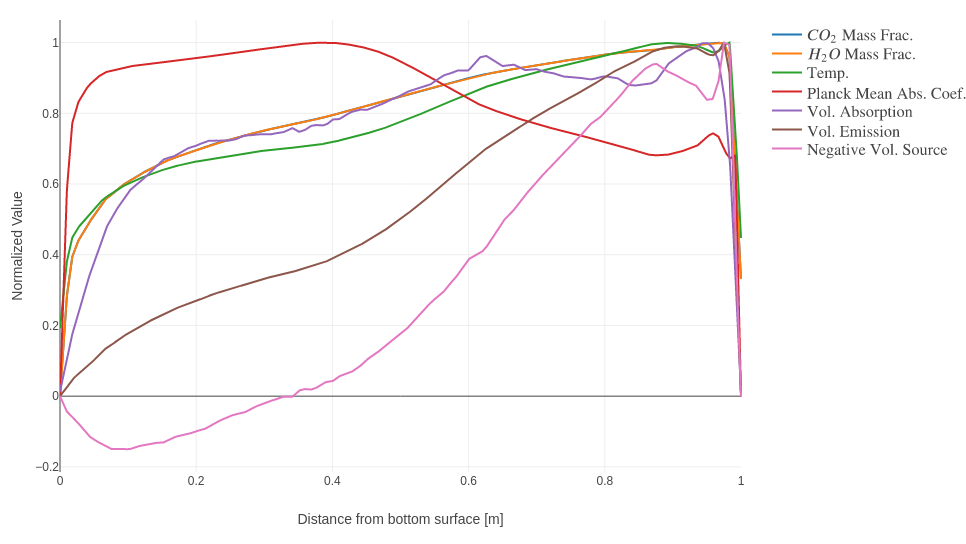
\includegraphics[width=\linewidth]{figures/ch4/line_plot_nongray.png}
% \caption{Various parameters along the center-line of a non-gray flame. Values normalized by maximum values along the sampled line.}
% \label{fig:PoolFire_lineplot_nongray}
% \end{figure}

\subsubsection{Transient simulation}
The pool-fire is simulated from initial conditions until 4 seconds of physical time.
The simulation is run with line-by-line accurate non-gray emission, and radiation source terms are updated each simulation time-step. Chemistry is infinitely-fast, and the case setup is identical to that of the frozen-field analysis.
The pool fire first appears as a mushroom near inlet, then the reacting, billowing cloud rises upwards, and finally exits through the top boundary of the domain.
The pool fire periodically fluctuates according to a \textit{puffing period}. These oscillations are buoyancy driven and result in turbulent eddies and substantial cooling of the flame as it mixes with the oxidizer.

Radiation contributes significantly to the reduction of flame temperature, and therefore has a significant effect on the density-driven buoyant forces fluctuating the flame profile. 
Figure \ref{fig:PoolFire_withandwithoutrad} compares the center-line temperature of the pool fire for a simulation without radiation, with the gray \verb|OpenFOAM-5.x| DOM radiation solver, and the gray MCRT model. Significant variations in temperature are apparent, up to $600$K at locations far from the inlet.


\begin{figure}
\centering
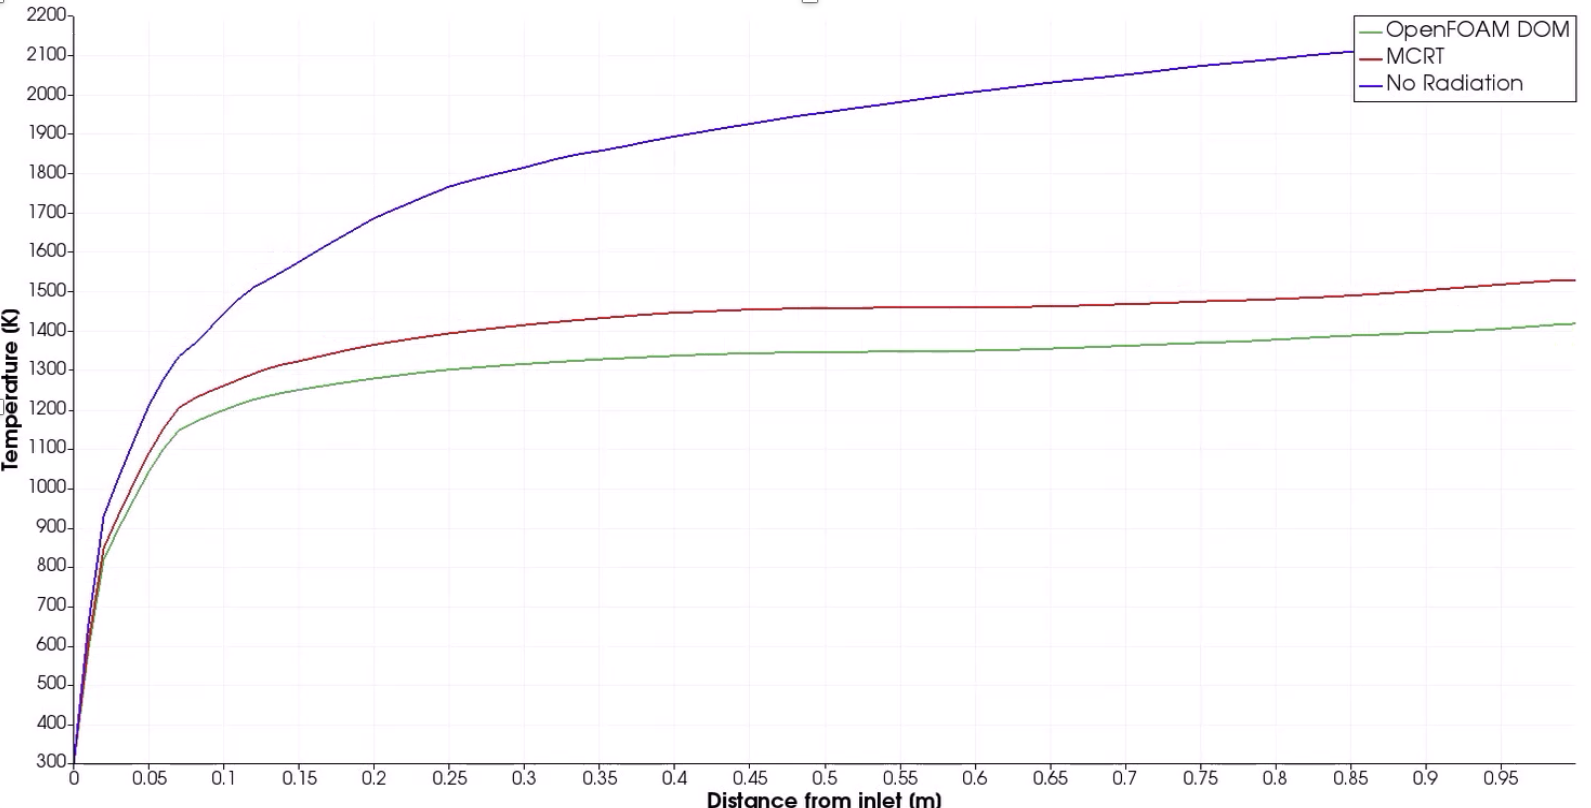
\includegraphics[width=0.7\linewidth]{figures/ch4/PoolFire_WithandWithoutRadiation.png}
\caption{Comparison of center-line temperature profiles of various simulations of the pool fire.}
\label{fig:PoolFire_withandwithoutrad}
\end{figure}

\subsection{Profiling}
\subsubsection{Single time-step}
The run-times of various sections of the radiation solver are presented in Figs.~\ref{fig:PoolFire_profiling} and \ref{fig:PoolFire_profiling_CPU} for both CPU and GPU simulations. Simulations are conducted with adaptive emission resulting in a total of 3,429,003 rays.
CPU ray-tracing is completed using 30 CPU processes. 

For both CPU and GPU simulations, the runtime is dominated by the loading of the non-gray database, which is over a gigabyte in size. 
The tracing region is proportionally smaller on the GPU as a result of the significant speedup when conducting raytracing in a SIMD-favorable architecture.
The loading process consists of first loading the data into memory, initializing the representative data structures, conducting various sanity checks on the database to ensure proper loading, and deep copying the data onto the GPU, if present.
Numerical time-step comparisons are present in Table \ref{table:PoolFireTimestep_runtime_table_1rpc}.

\begin{figure}
\centering
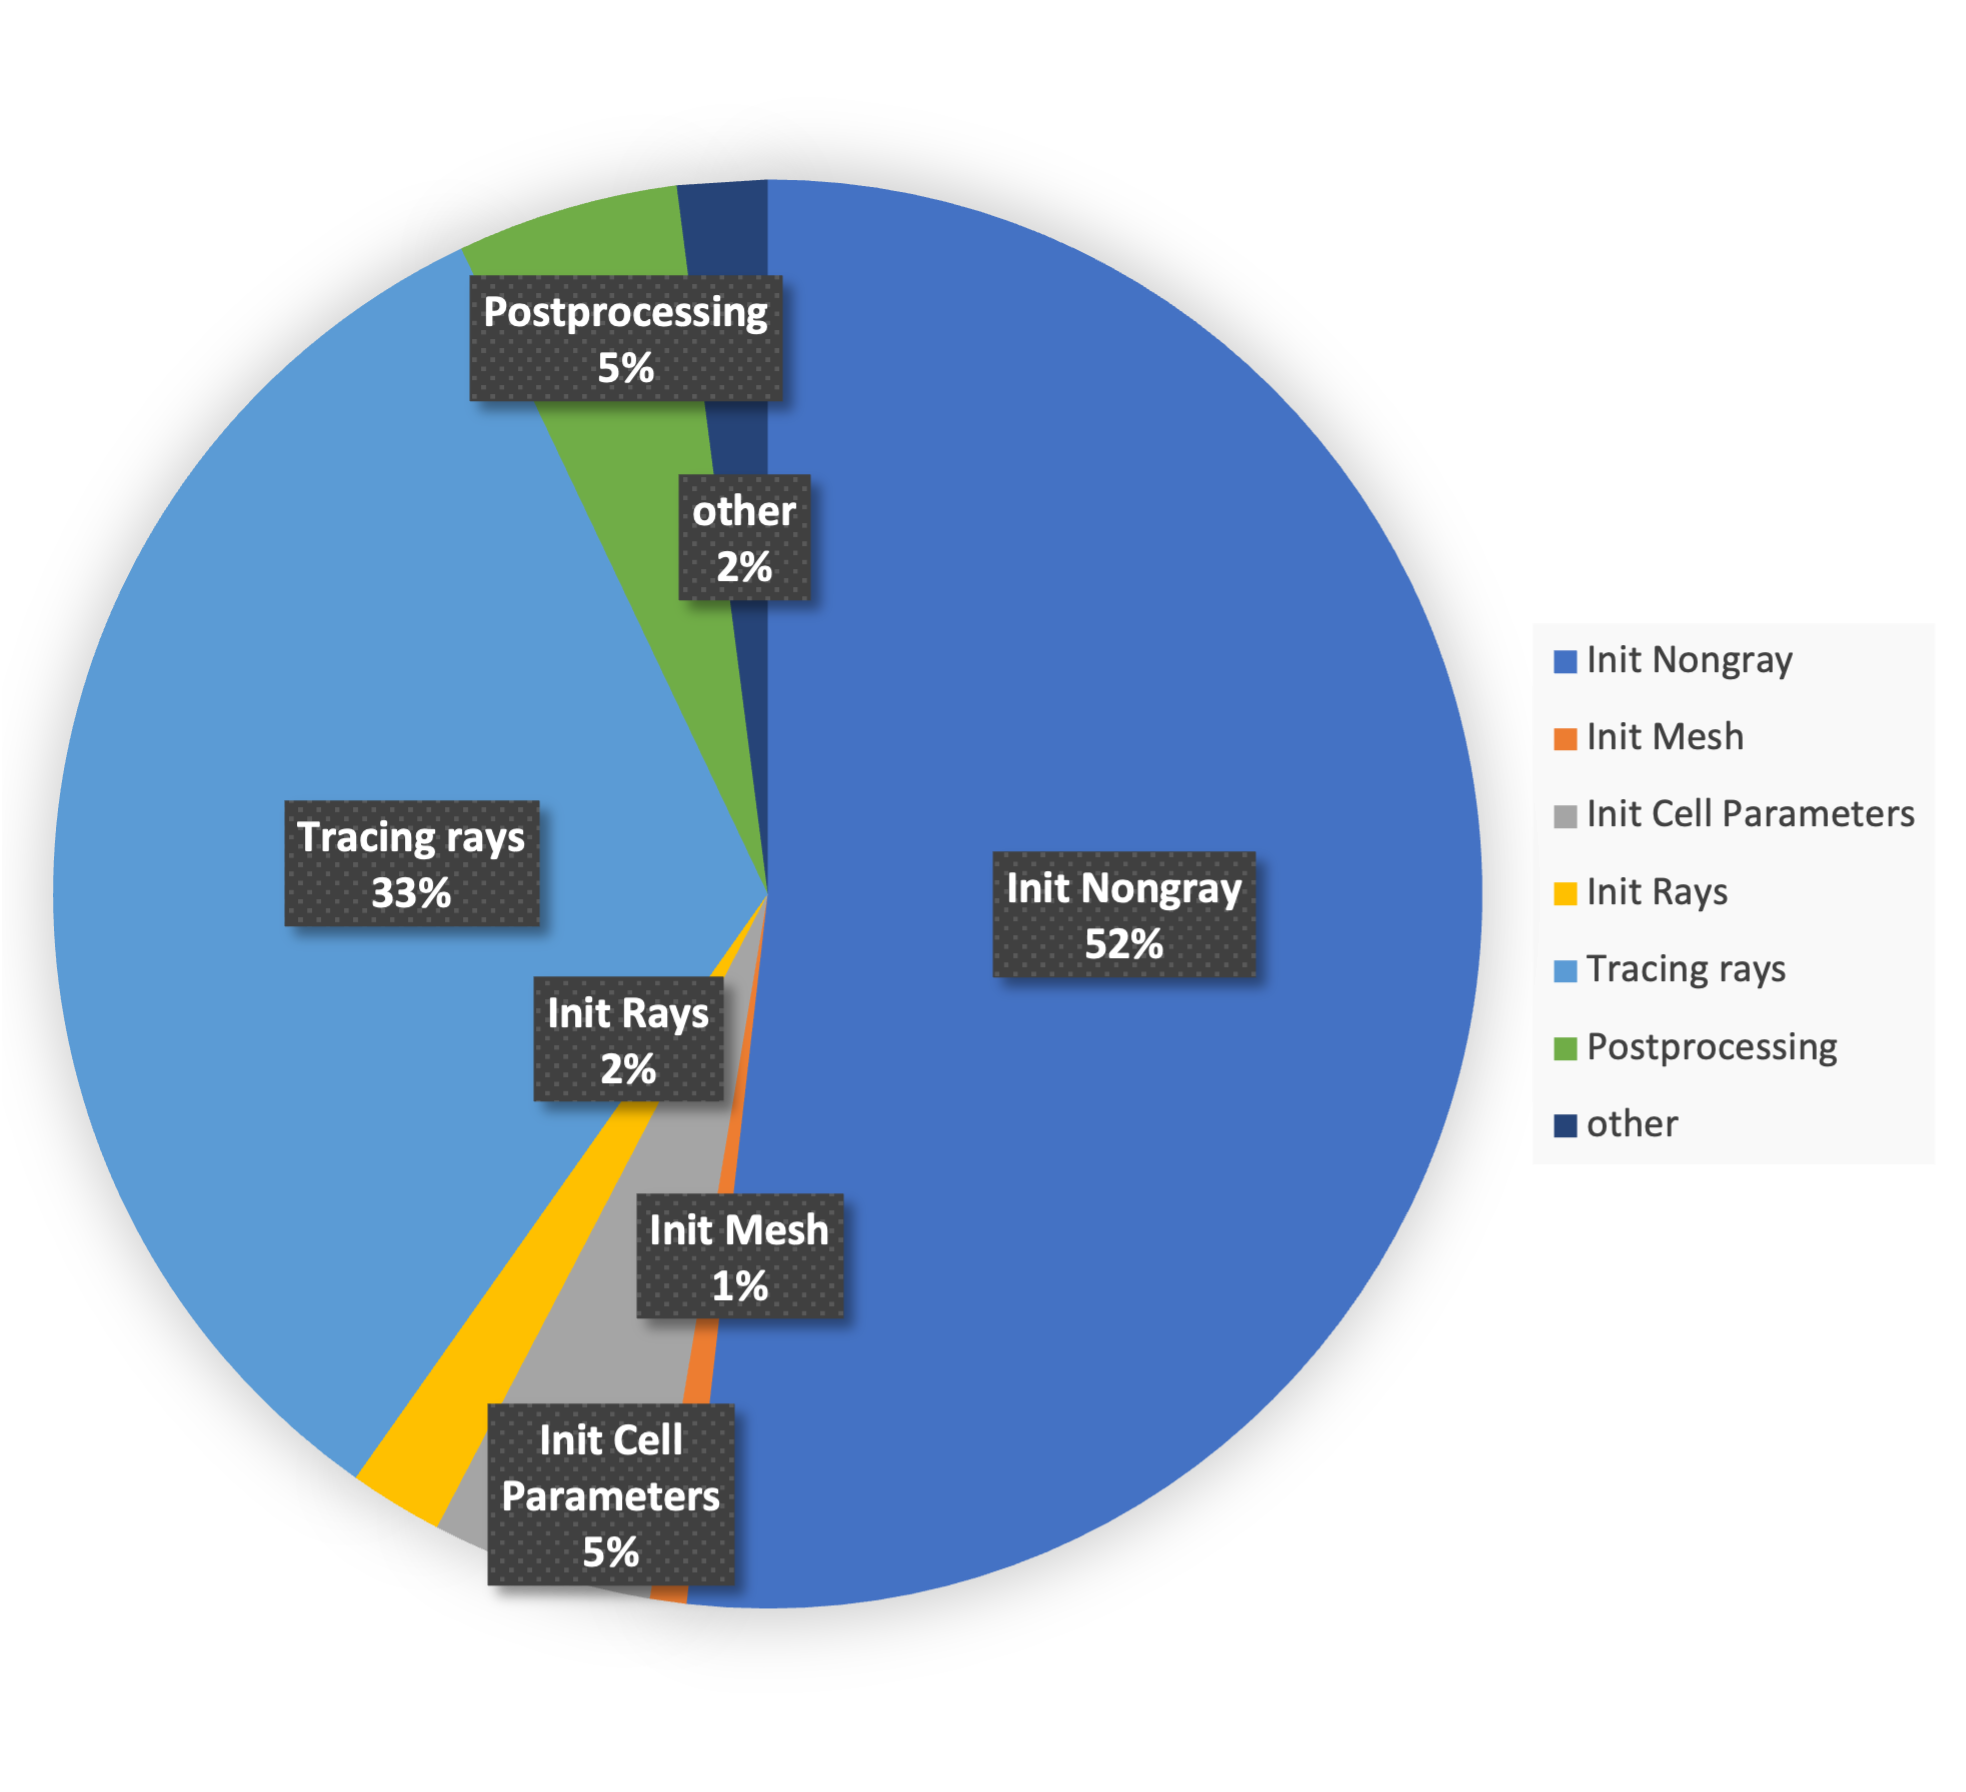
\includegraphics[width=0.675\linewidth]{figures/ch4/PoolFire_profiling_OnetimestepGPU.png}
\caption{Profiling results for the GPU}
\label{fig:PoolFire_profiling}
\end{figure}

\begin{figure}
\centering
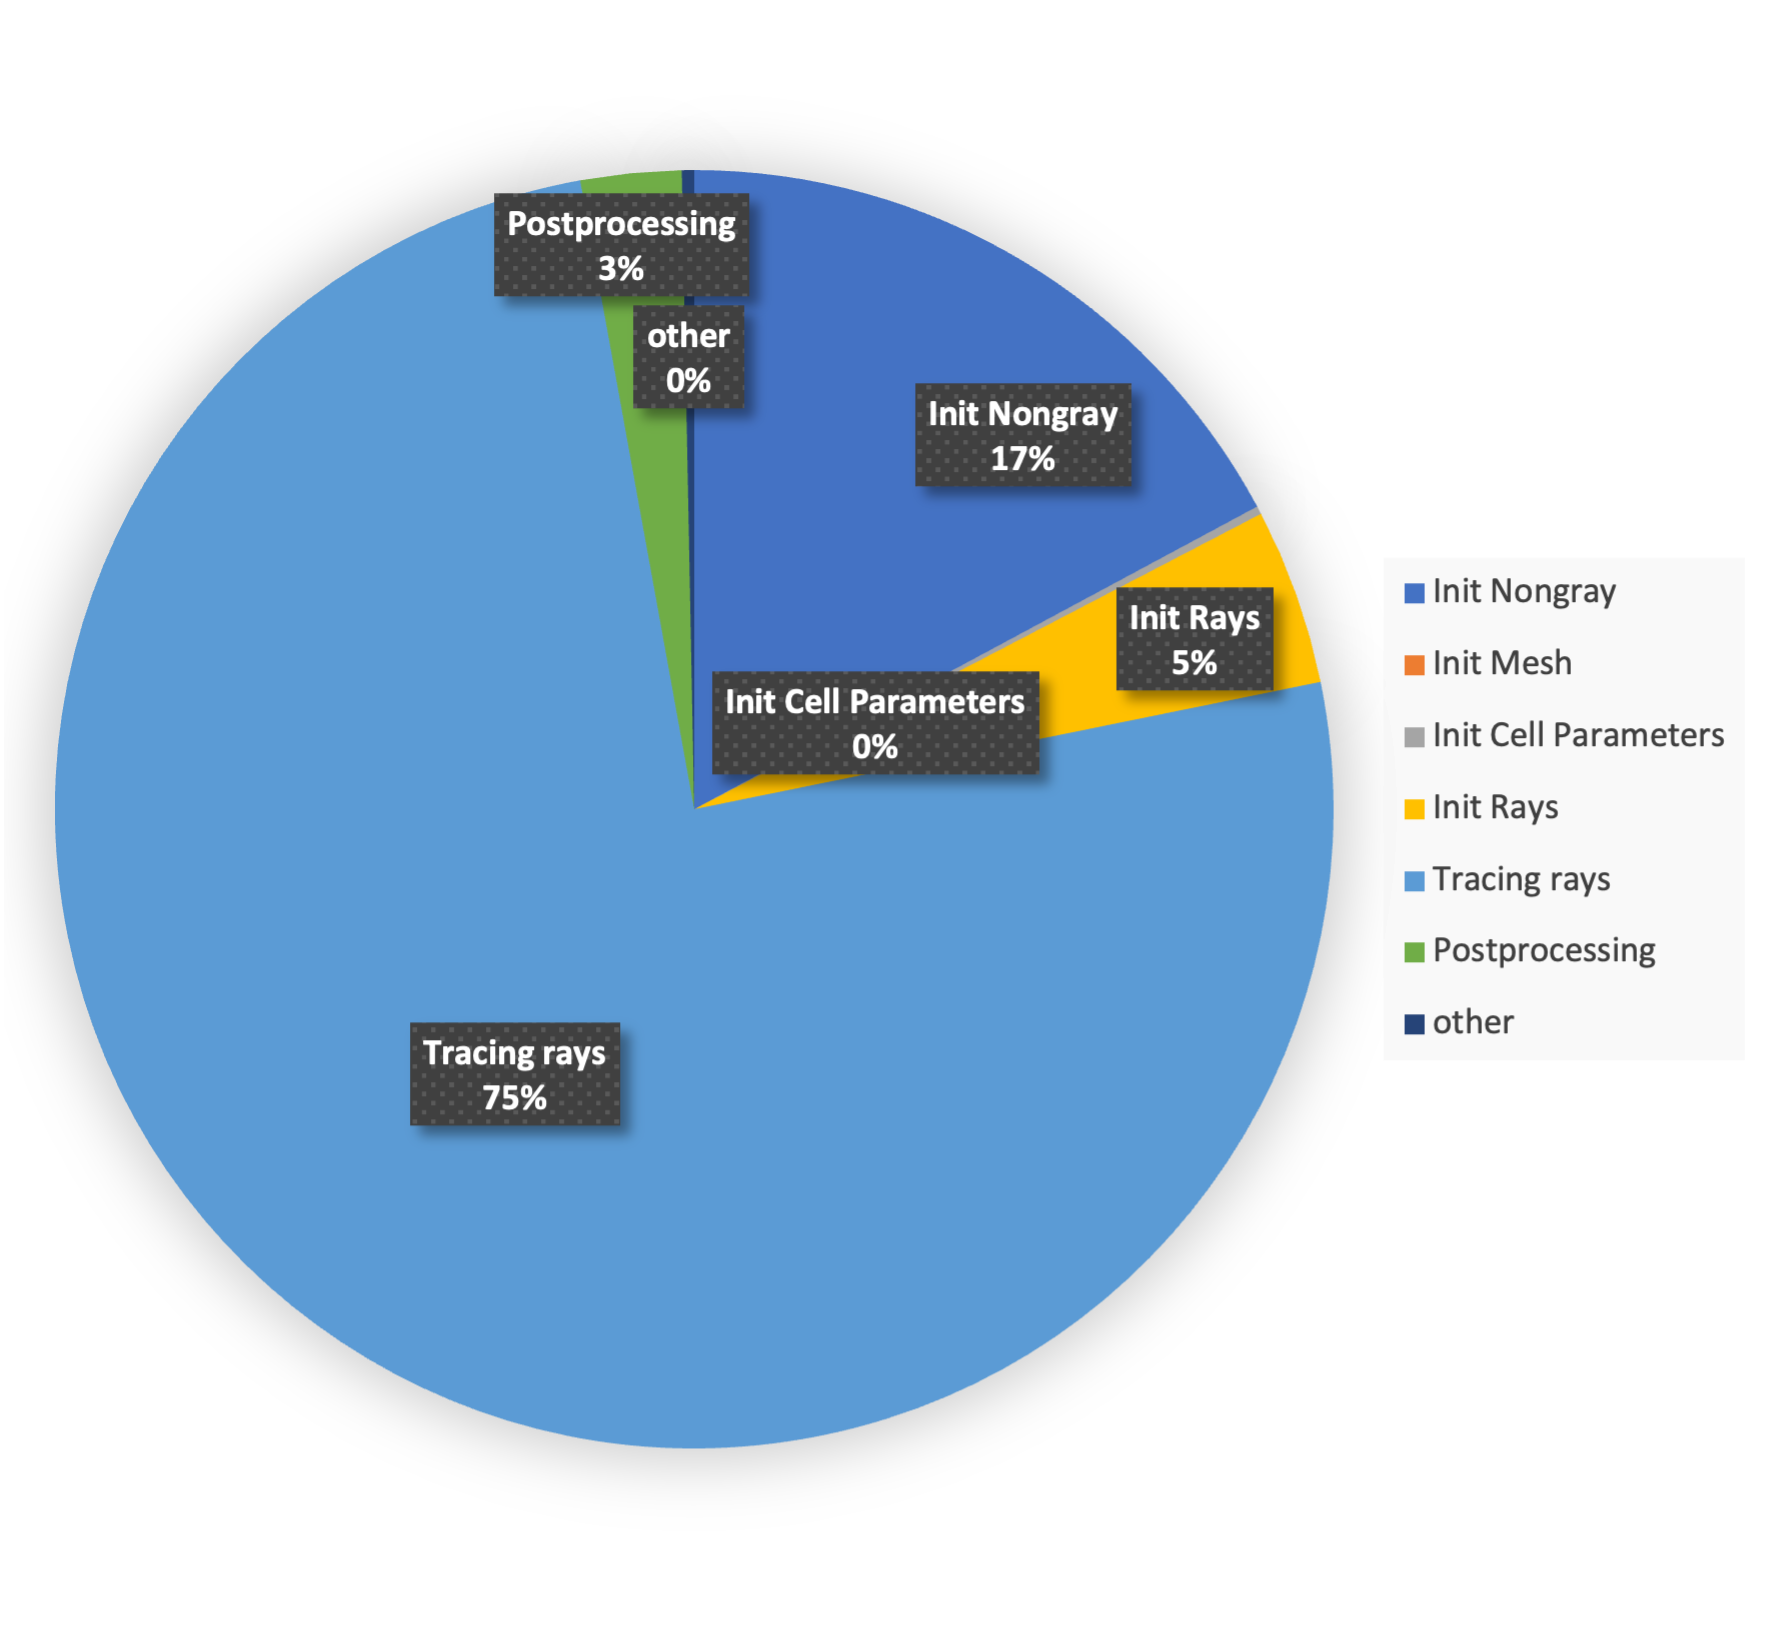
\includegraphics[width=0.675\linewidth]{figures/ch4/PoolFire_profiling_OnetimestepCPU.png}
\caption{Profiling results for the CPU.}
\label{fig:PoolFire_profiling_CPU}
\end{figure}

\begin{table}[h!]
\centering
\caption{Single time-step runtime profiling.}
\begin{tabular}{c c c c c} 
 \hline
 Parallel Variation & Init non-gray & Tracing rays & Init cell parameters & Total \\ [0.5ex] 
 \hline
 30 CPU processors & 0.997s & 4.38s & 0.0119s & 5.81s \\
 V100 GPU & 2.25s & 1.44s & 0.218s & 4.34s \\ 
 \hline
\end{tabular}
\label{table:PoolFireTimestep_runtime_table_1rpc}
\end{table}


\begin{table}[h!]
\centering
\caption{Mean runtime contribution of radiation per timestep compared to total runtime. Standard deviations are presented in parentheses. List CPU runtimes consist of radiation parallelized on 30 CPU processors, and CFD calculation occurring on 1 processor. GPU runtimes consist of radiation running on the GPU and CFD calculated using 1 CPU processor.}
\begin{tabular}{c c c c} 
 \hline
 Parallel Variation & Radiation Execution & Total Execution & Percent contribution \\ [0.5ex] 
 \hline
 30 CPU processors & 8.1s($\pm{}$0.58s) & 21.7s($\pm{}$0.84s) & 37.4\%($\pm{}$2.10\%) \\
 V100 GPU & 4.7s($\pm$0.28s) & 16.2s($\pm$2.21)s & 29.4\%($\pm$2.30\%) \\
 A100 GPU & 3.5s($\pm$0.10) & 14.1s($\pm$0.16)s & 24.8\%($\pm$0.70\%) \\
 \hline
\end{tabular}
\label{table:PoolFireTransient_runtime_table_1rpc}
\end{table}

\subsubsection{Transient simulation}
Transient simulations are  conducted with adaptive emission, totaling approximately 3,400,000 rays emitted and traced per time-step.
Both CPU and GPU versions were run for four seconds of simulation time. Mean and standard deviations of run-times are presented in table \ref{table:PoolFireTransient_runtime_table_1rpc}. 

For the CPU-run case, radiation encompassed approximately 37\% of the runtime for each timestep, on average.
It should be noted that both the non-gray database and CFD mesh are re-initialized every time step, resulting in significantly increased run-time. Future work will include initializing these components at the beginning of the simulation to prevent unnecessary overhead.
After these changes, it is projected that the overall radiation runtime targets approximately $6.7$~s, or $33$\% of the total runtime.
Similarly, the projected GPU runtime targets at $3.1$~s, or $21$\% of the total runtime per timestep.






